%% GreenFaaS: Carbon-Aware Scheduling for Serverless Workloads
%% Elsevier journal submission (review version, single column, line-numbered).
%%
%% To compile: ./build-elsevier.sh
%% To switch to camera-ready, change the document class option
%%   `review' -> `final' below.

\documentclass[review,12pt,authoryear]{elsevier/elsarticle}

% Tell LaTeX where to find the local copies of the class and BST files.
% (already loaded above; the BST file is referenced at the bottom.)

\usepackage{amsmath,amssymb,amsthm}
\usepackage{algorithm}
\usepackage{algpseudocode}
\usepackage{booktabs}
\usepackage{multirow}
\usepackage{graphicx}
\usepackage{xcolor}
\usepackage[T1]{fontenc}
\usepackage[hidelinks]{hyperref}
\usepackage{lineno}      % Elsevier expects line numbers on review submissions.
\linenumbers

% --- Tighter list spacing.
\usepackage{enumitem}
\setlist{itemsep=0.25ex,topsep=0.5ex,parsep=0.25ex}

% --- Theorem environment for Lemma 1.
\newtheorem{lemma}{Lemma}[section]
\newtheorem{theorem}[lemma]{Theorem}
\newtheorem{conjecture}[lemma]{Conjecture}

% --- Code-style font for short fragments.
\newcommand{\code}[1]{\texttt{\small #1}}

% --- Common notation shortcuts used in §4 and §5.
\newcommand{\GreenFaaS}{\textsc{GreenFaaS}}
\newcommand{\Interactive}{\textsc{Interactive}}
\newcommand{\Deferrable}{\textsc{Deferrable}}
\newcommand{\Background}{\textsc{Background}}

\journal{Future Generation Computer Systems}

\begin{document}

\begin{frontmatter}

\title{\GreenFaaS: Carbon-Aware Scheduling for Serverless Workloads}

% Single-anonymous review (FGCS default): author/affiliation block visible.
% For DOUBLE-anonymous review, comment this block out and uncomment the
% placeholder below.
\author[icosi]{Abdeldjalil Ledmi\corref{cor1}}
\ead{abdeldjalil.ledmi@univ-khenchela.dz}
\author[icosi]{Makhlouf Ledmi}
\ead{ledmi.makhlouf@univ-khenchela.dz}
\author[icosi]{Mohammed El Habib Souidi}
\ead{souidi.mohammed@univ-khenchela.dz}
\author[icosi]{Nabil Azizi}
\ead{azizi.nabil@univ-khenchela.dz}
\author[icosi]{Abdelkarim Oucif}
\ead{oucif.abdelkarim@univ-khenchela.dz}
\author[icosi]{Ferial Laassami}
\ead{ferial.laassami@univ-khenchela.dz}
\author[icosi]{Hichem Haouassi}
\ead{haouassi.hichem@univ-khenchela.dz}
\author[icosi]{Toufik Messaoud Maarouk}
\ead{maarouk.toufik@univ-khenchela.dz}

\affiliation[icosi]{organization={Department of Computer Science, ICOSI Lab, Abbes Laghrour University of Khenchela},
  city={Khenchela},
  postcode={40000},
  country={Algeria}}

\cortext[cor1]{Corresponding author.}

% --- Double-anonymous review placeholder (uncomment if required) ---
% \author{Anonymous Author(s)}
% \address{Affiliation withheld for double-anonymous review}

\begin{abstract}
Data centres' growing electricity footprint has motivated a body of
research on carbon-aware scheduling, in which workloads are shifted in
time or space to coincide with cleaner electricity. Much of the
foundational carbon-aware scheduling literature, however, targets
batch or long-running jobs, while recent FaaS-specific systems each
address only part of the spatial, temporal, hardware, and autoscaling
design space. The assumptions of the batch-oriented systems
--- minutes-to-hours runtime, delay tolerance, and clean
suspend/resume --- are profoundly violated by serverless or
Function-as-a-Service (FaaS) workloads. FaaS functions execute in
milliseconds to seconds, often under sub-second SLAs, suffer
expensive cold starts when interrupted, and arrive in bursty,
event-driven patterns.

We present \GreenFaaS, a carbon-aware scheduling framework for
serverless workloads that unifies three decisions previously treated
separately: spatial routing across regions, temporal deferral within
SLA bounds, and warm-pool-aware container reuse. Four prior FaaS-targeted
carbon-aware schedulers cover different facets of the design space:
\emph{GreenCourier} \citep{chadha2023greencourier} routes single
functions to low-carbon regions; \emph{Caribou} \citep{gsteiger2024caribou}
shifts whole serverless workflows geographically; \emph{EcoLife}
\citep{jiang2024ecolife} exploits multi-generation hardware; and
\emph{CASA} \citep{qi2024casa} co-optimizes autoscaling and SLOs within
a single cluster. \GreenFaaS{} is the first to give a closed-form
joint analysis of the spatial and temporal axes under cold-start
economics, and to demonstrate empirically-validated robustness across topology and
workload regimes.

The paper's principal analytical contribution is a closed-form
\emph{cold-start carbon trade-off}: we prove a dichotomy in which the
warm-pool placement decision is governed by a dimensionless idle-cost
ratio $\beta = P_i T_w / (P_a \tau_e)$ relative to a critical
threshold $(r-1)(1+\alpha)$, with a closed-form break-even condition and a unique critical
arrival rate $\lambda^*$ --- the root of a monotone scalar equation
--- separating the regimes. The same idle-cost ratio governs
the analogous temporal-shift trade-off with the deferral interval
$\Delta t$ in place of $T_w$, giving the scheduler principled
decision rules along both axes.

We evaluate \GreenFaaS{} in a discrete-event simulator, driven by a
schema-faithful synthetic workload calibrated to the Azure Functions
2019 and 2021 characterizations and by real grid carbon-intensity
data from Let's-Wait-Awhile \citep{wiesner2021lets,lwa} and from
ElectricityMaps over the same January 2021 window as the Azure trace,
against four carbon-aware baselines representative of recent work.
Three findings stand out.
\emph{First}, \GreenFaaS{} reduces operational carbon by 68--83\% relative to FIFO across
a range of topologies on fully-real time-aligned data (real Azure
2021 trace + real ElectricityMaps Jan 2021 carbon), and 64--72\% on
synthetic-workload setups. On fully-real time-aligned data the
\GreenFaaS{}--Spatial gap is 0.04 percentage points; across all
topologies on real-carbon data the gap stays within 0.5pp.
\GreenFaaS's distinct value over Spatial is topology-robustness
rather than dominance in any single regime.
\emph{Second}, \GreenFaaS{} preserves a \emph{do-no-harm} property
that extends beyond zero-opportunity workloads to a robust
neighbourhood of low-opportunity ones: across shiftable fractions
$\{0, 1\%, 2\%\}$ and in single-region scenarios on both synthetic
and fully-real data, \GreenFaaS{} matches FIFO byte-for-byte; a
heuristic ablation lacking the cold-start trade-off correction loses
5--102\% to FIFO in the same scenarios.
\emph{Third}, the canonical Wait-Awhile temporal scheduler and a
FaaS-adapted port of the provably-optimal one-way trading algorithm
of \citet{lechowicz2024online} both \emph{fail} on FaaS workloads,
losing 3--306\% to FIFO depending on the regime --- catastrophically
(up to $-306\%$) at batch-default deferral horizons on synthetic
workloads, and mildly (3--5\%) on fully-real data where they
degenerate toward a FIFO no-op. In neither regime do they reduce carbon: a clean
failure mode for batch carbon-aware techniques on FaaS, including
those with provable competitive guarantees, when warm-pool
idle-energy coupling is not accounted for. Head-to-head against the closest competing
serverless system, \emph{Caribou} \citep{gsteiger2024caribou}, well-tuned
Caribou (hourly re-deployment with perfect carbon forecasting) and
\GreenFaaS{} achieve statistically indistinguishable carbon savings (within 0.1pp) on real Azure
2021 workload; the difference is operational rather than empirical,
with \GreenFaaS{} avoiding the container migration and pub/sub
orchestration that Caribou requires.
The simulator, scheduler, trace loaders, Caribou port, and
real Azure Functions and ElectricityMaps integrations are released as
open-source artifacts under the Apache-2.0 license upon publication.

\end{abstract}

\begin{keyword}
carbon-aware scheduling \sep serverless \sep
Function-as-a-Service \sep cold start \sep sustainable computing
\end{keyword}

\end{frontmatter}

\section{Introduction}
\label{sec:introduction}

Data centres consume an increasing share of global electricity, and
hyperscale operators have made public commitments to carbon-neutral
or net-zero operation within the decade. These pledges have motivated
substantial research on \emph{carbon-aware computing}: techniques
that exploit spatial and temporal variation in grid carbon intensity
to shift computation toward cleaner energy. The dominant strategy in
the literature is \emph{temporal shifting} of delay-tolerant work to
periods of low carbon intensity \citep{wiesner2021lets}; complementary
\emph{spatial shifting} routes work toward regions with cleaner grids
\citep{sukprasert2023quantifying,radovanovic2023google}. Both have delivered
20--45\% operational-carbon reductions for batch processing, machine
learning training, and similar long-running workloads
\citep{hanafy2023carbonscaler,sukprasert2023quantifying}.

A critical assumption underlies essentially this entire body of work:
the target workload is \emph{batch} in character. The canonical
scheduled job is minutes to hours long, delay-tolerant on the order
of hours, amenable to clean suspend-and-resume, and accompanied by
enough up-front information that the scheduler can reason globally
over a set of pending jobs. These assumptions are violated profoundly
by \emph{serverless} or \emph{Function-as-a-Service} (FaaS) workloads,
which now power a substantial fraction of cloud-native applications.
FaaS invocations are typically measured in tens of milliseconds to a
few seconds; they are often user-facing with sub-second latency
objectives; they cannot be suspended and resumed without paying the
full cost of a \emph{cold start}; their arrivals are bursty and
event-driven; and per-invocation behaviour is largely unpredictable
until execution.

This mismatch is consequential. Recent FaaS-targeted carbon-aware
schedulers --- \emph{GreenCourier} \citep{chadha2023greencourier},
\emph{Caribou} \citep{gsteiger2024caribou}, \emph{EcoLife}
\citep{jiang2024ecolife}, and \emph{CASA} \citep{qi2024casa} --- have
each begun to address the gap from a distinct angle: spatial routing of
single functions (GreenCourier), workflow-level geo-shifting
(Caribou), hardware-generation choice (EcoLife), and SLO/carbon-aware
autoscaling (CASA). None of them, however, formalizes the joint
spatial/temporal/warm-pool decision problem that FaaS schedulers
actually face, and the fundamental cold-start versus idle-energy
trade-off has not previously been characterized in closed form.

We argue that carbon-aware scheduling for FaaS is both feasible and
distinct enough from its batch counterpart to warrant first-class
treatment. Three observations motivate our approach. \emph{First},
FaaS workloads are heterogeneous in latency tolerance: a
customer-facing API request demands sub-second response, but many
event-driven functions tolerate seconds to minutes of deferral
without observable user impact. \emph{Second}, FaaS platforms already
perform fine-grained placement and routing decisions for
load-balancing and cold-start mitigation; carbon-aware policies can
be layered onto this existing machinery. \emph{Third}, warm-pool
management --- how many idle containers to keep alive in each region
--- is itself a carbon decision, because idle containers consume
non-trivial power and the choice of where to keep them warm interacts
directly with the carbon intensity of the host grid.

In this work, we present \GreenFaaS, a carbon-aware scheduling
framework for serverless workloads that unifies spatial routing,
temporal deferral, and warm-pool-aware container reuse under a single principled
policy. \GreenFaaS{} combines temporal deferral for asynchronous and
event-driven invocations, spatial routing for latency-tolerant
classes, and carbon-aware warm-pool management, all under an
SLA-tiered policy distinguishing interactive, deferrable, and
background functions. A key technical contribution is the explicit
modelling of the \emph{cold-start carbon trade-off}: keeping
containers warm in a low-carbon region can, in some regimes, cost
more carbon (through idle power) than cold-starting in a
higher-carbon region. We derive analytical break-even points for
this trade-off and incorporate them directly into the scheduler.

We evaluate \GreenFaaS{} in \textbf{GreenFaaS-sim}, a discrete-event
simulator whose design follows the abstractions of \code{faas-sim}
and \code{vessim} \citep{faassim,vessim}, driven by the real Azure
Functions 2021 per-invocation trace
\citep{zhang2021faster,azuretrace} and by real grid carbon traces from
Let's-Wait-Awhile \citep{wiesner2021lets,lwa} and from
ElectricityMaps over the same January 2021 window as the Azure
trace. The trace loaders also accept a schema-faithful synthetic
workload as a fallback when the real trace is not locally available
(\S\ref{sec:evaluation:methodology}). We compare against four
carbon-aware baselines drawn from the recent literature, evaluating
along five axes: workload intensity, number of available regions, SLA
class mix, carbon-intensity variability, and forecast accuracy.

Our key findings are threefold. \emph{First}, \GreenFaaS{}
reduces operational carbon by 68--83\% across topologies on fully-real
time-aligned data (Azure 2021 trace + ElectricityMaps Jan 2021
carbon), and by 64--72\% on synthetic-workload setups; on fully-real
data the \GreenFaaS{}--Spatial gap is just 0.04 percentage points.
\emph{Second}, \GreenFaaS{} preserves a \emph{do-no-harm} property:
in single-region and flat-carbon regimes where shifting offers no
real opportunity, \GreenFaaS{} matches FIFO byte-for-byte on both
synthetic and fully-real data, while a heuristic ablation (lacking
the cold-start trade-off correction) loses 5--102\% to FIFO in the
same scenarios. \emph{Third}, the canonical Wait-Awhile temporal
scheduler and a FaaS-adapted port of the
\citet{lechowicz2024online} provably-optimal one-way trading
algorithm both \emph{fail} on FaaS workloads (3--306\% over FIFO
depending on the regime), an empirically sharp demonstration that
batch-oriented carbon-aware techniques --- including those with
provable competitive guarantees --- do not transfer to FaaS without
addressing warm-pool idle-energy coupling. This robustness across
regimes --- rather than dominance in any single regime --- is the
central practical claim of the paper.

\paragraph{Contributions.} The paper makes the following contributions:
\begin{enumerate}
\item A formal model of carbon-aware FaaS scheduling as an online
  optimization problem with capacity, SLA, and warm-pool constraints,
  and an honest discussion of why classical competitive-ratio bounds
  do not apply (\S\ref{sec:problem}).
\item A closed-form \emph{cold-start carbon trade-off lemma}
  characterizing warm-pool versus cold-start carbon as a function of
  arrival rate, runtime and cold-start durations, active and idle
  power, warm-pool TTL, and the carbon-intensity ratio between
  regions (\S\ref{sec:tradeoff}). The same dimensionless idle-cost
  ratio governs the analogous temporal-shift decision via an
  idle-energy correction (\S\ref{sec:tradeoff:idle}).
\item The \GreenFaaS{} scheduler: a hybrid online algorithm combining
  temporal deferral, spatial routing, and lemma-driven warm-pool
  management under an SLA-tiered policy, with $O(R \cdot N)$
  per-invocation cost (\S\ref{sec:algorithm}).
\item An open-source simulator with trace loaders that accept the
  published Azure Functions 2019, Azure Functions 2021, and LWA
  carbon-intensity schemas without modification
  (\S\ref{sec:simulator}).
\item An empirical evaluation against four carbon-aware baselines and
  a five-axis sensitivity sweep establishing the do-no-harm property
  across topology, SLA-class mix, forecast accuracy, carbon
  variability, and workload intensity (\S\ref{sec:evaluation}).
\end{enumerate}

The remainder of this paper is organized as follows.
\S\ref{sec:related} surveys related work; \S\ref{sec:motivation}
motivates the problem; \S\ref{sec:problem} formalizes it;
\S\ref{sec:tradeoff} derives the trade-off lemma;
\S\ref{sec:algorithm} presents the algorithm; \S\ref{sec:simulator}
describes the simulator; \S\ref{sec:evaluation} reports results;
\S\ref{sec:discussion} discusses limitations; \S\ref{sec:conclusion}
concludes.

\section{Related Work}
\label{sec:related}

Carbon-aware scheduling has matured rapidly over the past four years.
We organise prior work into four threads: (i) batch and long-running
workloads, where the dominant approaches assume delay-tolerance and
suspend/resume; (ii) theoretical foundations of online carbon-aware
scheduling; (iii) the small but growing set of carbon-aware
schedulers explicitly targeting serverless or FaaS workloads, with
which \GreenFaaS{} most directly engages; and (iv) FaaS systems work
on cold-starts, warm pools, and characterization, on which our cost
model depends.

\subsection{Carbon-Aware Scheduling for Batch Workloads}

Wiesner et al.'s \emph{Let's Wait Awhile} \citep{wiesner2021lets}
introduced threshold-based deferral for batch workloads and released
the hourly carbon-intensity dataset (DE, GB, FR, US-CAISO, 2020) that
has become the de-facto reference; we use this dataset directly in
our evaluation (\S\ref{sec:evaluation:methodology}).
\emph{CarbonScaler} \citep{hanafy2023carbonscaler} scales the
parallelism of ML training jobs in response to carbon intensity,
exploiting the elasticity of data-parallel workloads.
Souza et al.'s \emph{GAIA} scheduler
\citep{sukprasert2023quantifying} addresses the three-way trade-off
between carbon, performance, and cost for batch jobs, and quantifies
the practical limits of carbon-aware spatiotemporal shifting; the same
group's \emph{Ecovisor} \citep{souza2023ecovisor} provides a virtual
energy system abstraction. Google's Carbon-Intelligent Compute
\citep{radovanovic2023google} deploys a Variable Capacity Curve
approach at production scale.
\emph{LACS} \citep{bostandoost2024lacs} is a learning-augmented
resource scaler addressing uncertain demand.
\emph{Adapting Datacenter Capacity} \citep{lin2023adapting} explored
provisioning to track grid carbon.

These works share two structural assumptions that \GreenFaaS{}
relaxes. \emph{First}, the schedulable units are \emph{jobs} with
cost separable per-job, allowing the schedulers to reason about each
job's deferral in isolation. FaaS invocations are not separable in
this sense because their cost is coupled through warm-pool state,
which we formalize in \S\ref{sec:problem}. \emph{Second}, the
schedulers operate on a timescale (minutes to hours) where cold-start
penalties are negligible. We show empirically in
\S\ref{sec:evaluation} that naively transplanting these techniques to
FaaS workloads --- as the Wait-Awhile baseline does ---
\emph{more than doubles} operational carbon relative to a
carbon-unaware FIFO baseline (163--236\% above FIFO across our
synthetic and real-carbon experiments). The ``batch schedulers don't
transfer'' claim is therefore not only intuitively obvious from the
assumption mismatch but also empirically severe.

\subsection{Theoretical Foundations}

A recent line of work has put carbon-aware online algorithms on
firmer footing. Lechowicz et al.'s \emph{Online Pause and Resume
Problem} \citep{lechowicz2024online} studies a one-dimensional model
in which a workload can be paused during high-carbon periods and
resumed during low-carbon periods, paying a fixed switching cost.
They derive double-threshold algorithms with provably optimal
competitive ratios. These theoretical results apply to a workload
model that is in several respects strictly simpler than ours: a
single workload (no multi-tenant mix), one machine (no spatial
routing), and a single switching cost (no idle-energy accumulation).
The FaaS setting we study introduces three structural features ---
per-invocation cold-start versus warm-pool trade-offs, spatial
routing across regions, and tiered SLA constraints --- that take us
outside the class of problems for which competitive-ratio bounds are
currently known. We are explicit in \S\ref{sec:problem:online} that
\GreenFaaS{} is an empirical scheduler with a \emph{local}
analytical guarantee (Lemma~\ref{lemma:tradeoff}'s break-even
characterization) rather than a competitively-optimal one. Extending
\citep{lechowicz2024online} to handle warm-pool idle energy and SLA
tiering is an open direction we identify in \S\ref{sec:discussion}.

\subsection{Carbon-Aware FaaS and Serverless}
\label{sec:related:faas}

Five recent systems target serverless workloads specifically; each
covers a different facet of the design space.

\paragraph{GreenCourier \citep{chadha2023greencourier}.} The closest
single-function spatial-routing precedent: a Kubernetes scheduler
plugin that routes serverless functions across geographically
distributed Knative clusters based on real-time grid carbon intensity.
It reports 9--18\% carbon reduction per invocation with negligible
latency overhead. GreenCourier and \GreenFaaS{} share the high-level
goal but differ in three significant respects.
\emph{First}, GreenCourier is \emph{spatial-only} --- it routes
functions to the cleanest available region, with no temporal deferral
and no warm-pool reasoning. Our headline contribution beyond
GreenCourier is therefore the joint spatial/temporal/warm-pool policy
and the underlying trade-off analysis.
\emph{Second}, GreenCourier has no analytical model of the warm-pool
versus cold-start carbon trade-off; our Lemma~\ref{lemma:tradeoff}
gives a closed-form characterization that becomes essential as soon
as the scheduler reasons about \emph{whether} to maintain a warm
pool.
\emph{Third}, GreenCourier's reported savings (9--18\%) sit at the
lower end of what our headline results suggest is achievable; we
attribute this to the spatial-only scope rather than to algorithmic
deficiencies in GreenCourier itself.

\paragraph{Caribou \citep{gsteiger2024caribou}.} Caribou is the
closest recent system in scope at the workflow level. It offloads
serverless \emph{workflows} (multi-function DAGs) across
geo-distributed regions for sustainability, automatically
(re-)deploying functions and redirecting traffic to lower-carbon
endpoints. Caribou requires no changes to application logic and
preserves performance and cost metrics. Its scope is workflow-level
spatial (no temporal deferral, no per-invocation warm-pool
reasoning), with decisions made at deployment time and refreshed by
periodic redeployment rather than per invocation.

We compare head-to-head in \S\ref{sec:evaluation:caribou} by porting
Caribou's deployment-solver logic to our per-invocation workload as
a single-node DAG case, with perfect carbon forecasting and constant
token-bucket grant (both favourable to Caribou). The finding:
Caribou(1h) and \GreenFaaS{} achieve carbon savings that differ by less than 0.1 percentage points
on our 24h FaaS slices; the two systems are operationally distinct
but empirically equivalent on per-invocation workloads with hour-scale
carbon variation. The systems are complementary along the granularity
axis: Caribou makes coarse-grained, deployment-time placement decisions
for whole workflows; \GreenFaaS{} makes fine-grained, per-invocation
decisions including warm-pool reasoning. A natural composition would
use Caribou for workflow placement and \GreenFaaS{} for per-invocation
scheduling within each chosen region; we have not implemented this
composition.

\paragraph{EcoLife \citep{jiang2024ecolife}.} EcoLife targets the
hardware-generation axis: it co-optimizes \emph{operational} and
\emph{embodied} carbon by exploiting multi-generation hardware (newer
servers are faster but have higher embodied carbon per unit time;
older servers are slower but already amortised). It uses a Particle
Swarm Optimisation-based scheduler that decides, per invocation, which
hardware generation to execute on. EcoLife explicitly reasons about
keep-alive (warm-pool) versus cold-start trade-offs --- which makes
it the closest precedent for our Lemma~\ref{lemma:tradeoff} --- but
it does so through a metaheuristic optimizer without a closed-form
characterization. The two contributions are largely orthogonal:
EcoLife answers ``on what hardware generation should this function
execute?''; \GreenFaaS{} answers ``in what region and at what time
should this function execute, and is a warm pool worth maintaining
there?''. A scheduler combining the two axes is a natural follow-up
(\S\ref{sec:discussion:embodied}).

\paragraph{CASA \citep{qi2024casa}.} CASA is the closest recent
single-cluster, autoscaling-focused competitor. It is an SLO- and
carbon-aware framework that schedules and autoscales containers in a
serverless cluster, explicitly trading off the SLO cost of cold-starts
against the carbon cost of pre-warming and keep-alive. CASA reports up
to a $2.6\times$ reduction in operational carbon while reducing SLO
violations by up to $1.4\times$ over a state-of-the-art baseline. The
follow-on work \citep{qi2024wastewater} extends the same multi-objective
framework to co-optimize wastewater alongside carbon and SLOs. CASA
and \GreenFaaS{} address overlapping concerns through different
mechanisms. CASA's contribution is a carbon-aware autoscaling and
container-placement policy in a single cluster, evaluated by simulation
against a state-of-the-art autoscaler. \GreenFaaS's contribution is a
closed-form trade-off characterization
(Lemma~\ref{lemma:tradeoff}) that yields a parameter-free per-invocation
decision rule, combined with a multi-region routing policy and a
formal do-no-harm property
(\S\ref{sec:evaluation:topology},
\S\ref{sec:evaluation:realtopology}). Where CASA establishes that
carbon-aware autoscaling is worthwhile, \GreenFaaS{} establishes the
analytical conditions under which warm-pool maintenance is itself
carbon-positive --- a question CASA's heuristics do not pose
explicitly. The two approaches could be composed at different
granularities: CASA at the container-pool autoscaling layer, \GreenFaaS{}
at the per-invocation routing-and-warm-pool-gate layer.

\paragraph{GreenWhisk \citep{greenwhisk}.} GreenWhisk is a
system-level redesign of Apache OpenWhisk to expose energy and carbon
state to load-balancing algorithms, supporting both grid-connected and
grid-isolated modes. Its contribution is infrastructural: an
energy-interface API and a carbon-aware load-balancer integrated into
a production-grade FaaS platform. The scheduling algorithm itself is
intentionally minimal in scope; the value is the open-platform
abstraction. \GreenFaaS's algorithmic and analytical contributions are
compatible with this abstraction: a production GreenWhisk deployment
could load Algorithm~\ref{alg:greenfaas} as its load-balancing policy
without changes to either side. GreenWhisk's two-mode design (grid
intermittency) is a deployment dimension our analysis does not address
and that an integration would have to handle separately.

\paragraph{CASPER \citep{souza2024casper}.} Adjacent rather than
directly competing: targets distributed web services (MediaWiki-class
applications) under latency SLOs, using a mixed-integer program to
jointly provision servers and load-balance requests across cloud
regions. It addresses spatial routing and provisioning with SLO
constraints but treats requests at the application level (request
rates, not per-invocation arrivals) and does not engage with
cold-start economics. We position \GreenFaaS{} as the per-invocation,
FaaS-native analogue of CASPER, with the cold-start trade-off model as
a key technical distinction.

\subsection{Serverless Cold-Starts and Characterisation}

Our cost model in \S\ref{sec:problem} and the SLA-tiered policy in
\S\ref{sec:algorithm:sla} depend on a substantial body of FaaS
systems work. \emph{Serverless in the Wild}
\citep{shahrad2020serverless} is the canonical characterization of
production Azure Functions workloads; it established that
invocations are dominated by a small number of high-frequency
``hot'' functions, that durations follow heavy-tailed distributions,
and that arrival processes are bursty and event-driven. Our workload
generator and the function popularity model (Zipf with $s = 1.2$)
follow this characterization directly. The follow-up
\emph{Azure Functions Invocation Trace 2021}
\citep{zhang2021faster,azuretrace} gives per-invocation records over
two weeks; we use its schema as the basis for our trace loader
(\S\ref{sec:evaluation:methodology}).

The cold-start problem itself has a rich literature.
\emph{Catalyzer} \citep{du2020catalyzer} and \emph{Firecracker}
\citep{agache2020firecracker} attack cold-starts at the system level
via micro-VM and snapshot techniques. \emph{FaaSCache}
\citep{fuerst2021faascache} frames warm-pool management as a caching
problem and derives keep-alive policies from caching theory. We
borrow the warm-pool / keep-alive abstraction directly, but add the
carbon dimension: idle energy at intensity $C_r$ in region $r$ is
itself a cost that the scheduler must trade off against cold-start
energy at potentially different $C$. This is the substance of our
Lemma~\ref{lemma:tradeoff}.

A parallel measurement-focused line of work makes it possible to
attribute per-invocation carbon footprints to FaaS workloads with
high accuracy. \emph{Accountable Carbon Footprints}
\citep{sharma2024accountable} develops a Shapley-value-based
disaggregation methodology that fairly attributes shared hardware and
software emissions to individual function invocations, achieving
$>$99\% accuracy on a wide range of workloads. This work is
methodologically orthogonal --- it measures, we schedule --- but a
production-grade carbon-aware scheduler should integrate with such a
measurement substrate to close the loop from decisions to observed
outcomes.

\paragraph{Summary of positioning.} To our knowledge, no prior work
has formalized the cold-start carbon trade-off in closed form,
demonstrated the temporal-axis idle-energy correction
(\S\ref{sec:tradeoff:idle}), or established a do-no-harm property
across topology, SLA-mix, forecast-accuracy, and carbon-variability
axes. These are the empirical and analytical novelties on which the
rest of the paper builds.

\section{Motivation}
\label{sec:motivation}

We motivate carbon-aware FaaS scheduling with a joint characterization
of the two data sources that drive our design: a representative FaaS
workload, and the grid carbon-intensity signal that determines the
carbon footprint of executing that workload.

\subsection{Joint Characterisation}

Figure~\ref{fig:motivation} overlays a 48-hour grid carbon-intensity
trace for Germany --- a synthetic trace whose annual mean is
calibrated to the ENTSO-E 2020 figure later validated against real
LWA data in \S\ref{sec:evaluation:realcarbon} --- with the per-minute
invocation rate of a representative \code{webhook\_handler} function
drawn from a workload generator calibrated to the
\citet{shahrad2020serverless} Azure characterization. Shaded bands
mark the lowest-quartile (green) and highest-quartile (red) carbon
windows over the 48-hour horizon. Three observations emerge.

\begin{figure*}[t]
\centering
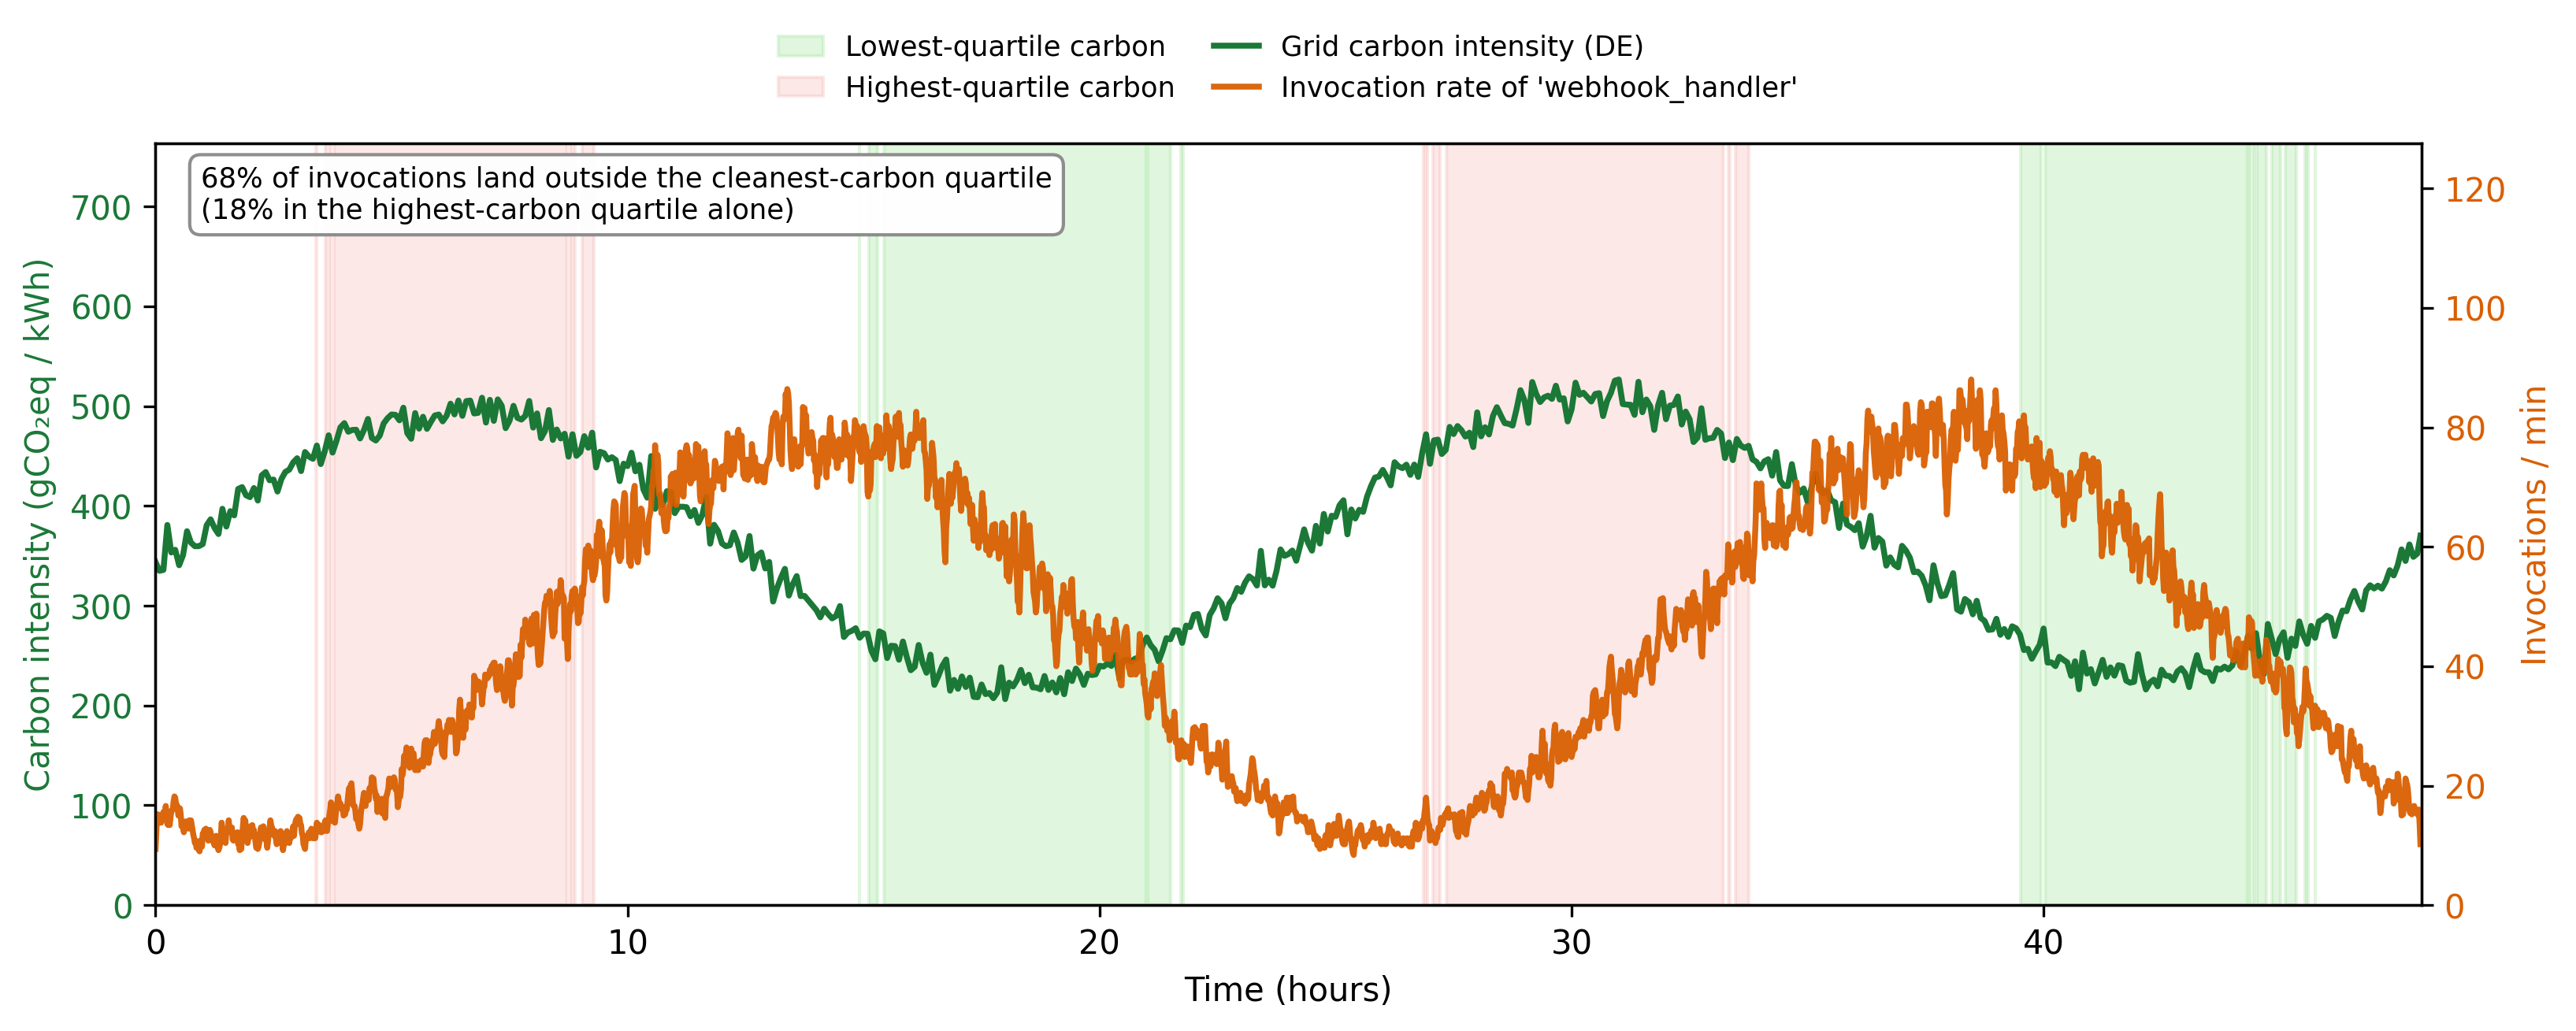
\includegraphics[width=0.95\textwidth]{figures/motivation_carbon_vs_invocations.png}
\caption{FaaS arrivals are decoupled from grid carbon intensity. The
orange line (right axis) shows the per-minute invocation rate of the
\code{webhook\_handler} function; the green line (left axis) shows
grid carbon intensity in Germany. The two signals are phase-shifted by
8--12 hours, creating temporal shifting opportunity for deferrable
invocations. Shaded bands mark the lowest- (green) and highest-carbon
(red) quartile windows.}
\label{fig:motivation}
\end{figure*}

\paragraph{1. FaaS arrival rates are decoupled from grid carbon
intensity.} The webhook function's rate follows a business-hours
diurnal pattern, peaking in early afternoon and troughing overnight.
Grid carbon intensity in Germany follows the inverse pattern: solar
and wind generation peak around midday, depressing the marginal
intensity, while night-time demand is served by base-load fossil
generation. The two signals are phase-shifted by roughly 8--12 hours;
on this representative day, 68\% of webhook invocations land
\emph{outside} the cleanest carbon quartile and 18\% land directly
in the highest-carbon quartile. The decoupling is the structural
reason carbon-aware scheduling can help.

\paragraph{2. The decoupling is robust across function classes.}
Across the 60-function catalog generated for our evaluation, the
population-weighted invocation rate correlates only weakly with the
local carbon intensity (Pearson $r$ in the range $-0.2$ to $+0.1$
across regions), confirming that arrival patterns track user activity
rather than grid economics --- as expected, since FaaS workloads are
driven by external events (user requests, message-queue depths,
scheduled triggers) that have no relationship to the regional
generation mix.

\paragraph{3. The amplitude of the carbon swing is comparable to the
amplitude of the arrival swing.} Carbon intensity in Germany swings
from $\sim$200 to $\sim$500 gCO$_2$eq/kWh over the 24-hour cycle ---
a ratio of $2.5\times$. The webhook invocation rate swings from
$\sim$15 to $\sim$80 invocations per minute --- a ratio of
$5\times$. The two signals have similar dynamic range, which means a
scheduler that can shift even a modest fraction of invocations
across the diurnal cycle has potential to capture meaningful savings.
We quantify this potential rigorously in \S\ref{sec:evaluation}.

\subsection{Implications for Scheduler Design}

The characterization directly motivates three design choices in
\S\ref{sec:algorithm}. \emph{First}, the SLA-tiered policy: arrivals
distributed across the carbon cycle are only useful to a scheduler
that distinguishes between invocations that must execute immediately
(interactive) and those that can wait. \emph{Second}, the use of
\emph{both} spatial and temporal axes: a purely temporal scheduler can
only exploit the diurnal swing within one region; a purely spatial
scheduler ignores the substantial within-region opportunity
Figure~\ref{fig:motivation} reveals. \emph{Third}, the explicit
carbon-aware warm-pool reasoning of \S\ref{sec:tradeoff}: at the
timescale of FaaS invocations (seconds), the idle-energy cost of
keeping containers warm is a first-class concern.

The motivation, in short, is not ``carbon-aware scheduling helps
FaaS'' in some generic sense --- that has been shown by the four
FaaS-targeted systems surveyed in \S\ref{sec:related:faas}
\citep{chadha2023greencourier,gsteiger2024caribou,jiang2024ecolife,qi2024casa}.
The motivation is that the \emph{specific structure} of FaaS
workloads (short, bursty, latency-tiered) combined with the
\emph{specific structure} of grid carbon traces (diurnal, decoupled
from user activity, multi-region heterogeneous) creates a joint
optimization problem that no prior scheduler has addressed in its
full generality. The rest of the paper formalizes and solves that
problem.

\section{Problem Formulation}
\label{sec:problem}

This section formalizes the carbon-aware FaaS scheduling problem.
\S\ref{sec:problem:statement} sets up the entities, decision variables,
and constraints. \S\ref{sec:problem:online} frames the optimization as
an online problem and discusses why it admits neither a tractable
offline optimum nor a competitive-ratio bound, motivating the
empirical evaluation strategy in \S\ref{sec:evaluation}.

\subsection{Problem Statement}
\label{sec:problem:statement}

\paragraph{Regions.} A set $\mathcal{R} = \{r_1, \ldots, r_R\}$ of
geographic regions. Each region $r$ has capacity $K_r$, a time-varying
grid carbon intensity $C_r: \mathbb{R}_{\ge 0} \to \mathbb{R}_{>0}$
in gCO$_2$eq/kWh, a Power Usage Effectiveness $\mathrm{PUE}_r \ge 1$,
and network round-trip latencies $\rho(r, r') \ge 0$ to every other
region.

\paragraph{Functions.} A set $\mathcal{F}$ of deployed functions, each
$f \in \mathcal{F}$ characterized by expected execution time
$\tau_e(f)$, cold-start duration $\tau_c(f)$, active power $P_a(f)$,
idle power $P_i(f)$, latency class
$\ell(f) \in \{\Interactive, \Deferrable, \Background\}$, and SLA
deadline $D(f)$. The latency class determines the scheduler's degree
of freedom: \Interactive{} invocations must execute immediately in
their home region; \Deferrable{} invocations may be deferred up to a
class-dependent horizon and routed within a tight RTT budget;
\Background{} invocations may use their full deadline and any region.

\paragraph{Invocations.} Function invocations arrive as a stream
$\mathcal{I} = \langle i_1, i_2, \ldots \rangle$ ordered by arrival
time. Each $i$ specifies a function $f(i)$, an arrival time $a(i)$, a
home region $h(i)$, and a realised runtime $\tau(i)$ drawn from
$f(i)$'s execution-time distribution. Crucially, $\tau(i)$ is
\emph{not} known to the scheduler at decision time; only the
expected runtime $\tau_e(f(i))$ is. The same applies to future
arrivals: at time $a(i)$ the scheduler sees $i$ but knows nothing
about $i_k$ for $k$ with $a(i_k) > a(i)$ beyond what an arrival-rate
estimator can infer.

\paragraph{Warm pools.} For each $(r, f) \in \mathcal{R} \times
\mathcal{F}$, the platform maintains a non-negative integer
warm-container count $W_{r,f}(t)$ representing containers that have
previously executed $f$ in $r$ and remain alive awaiting reuse. A
warm container is evicted after a TTL of $T_w$ seconds of inactivity.

\paragraph{Decisions.} For each invocation $i$, the scheduler produces
$\pi(i) = (r(i), s(i))$: the execution region $r(i)$ and the
scheduled start time $s(i)$. The secondary outcome
$w(i) = \mathbf{1}[W_{r(i), f(i)}(s(i)) > 0]$ --- whether $i$ finds a
warm container at $r(i)$ at time $s(i)$ --- is observed rather than
chosen; if $w(i) = 0$, the invocation pays $\tau_c(f(i))$ in
start-up latency and energy.

\paragraph{Per-invocation cost.} The carbon cost of $i$ under
$\pi(i) = (r, s)$ is
\begin{equation*}
\mathrm{Carbon}(i) = \tfrac{\mathrm{PUE}_r}{3.6 \times 10^6}\,C_r(s)
\cdot P_a(f(i))\big[\tau(i) + (1-w(i))\tau_c(f(i))\big].
\end{equation*}
End-to-end latency is
\begin{equation*}
\mathrm{Lat}(i) = (s - a(i)) + \rho(h(i), r) + (1-w(i))\tau_c(f(i)) + \tau(i).
\end{equation*}

\paragraph{System cost.}
\label{sec:problem:cost}
Aggregate carbon over horizon $[0, T]$ sums
per-invocation execution carbon and warm-pool idle carbon. The exact
idle carbon integrates the time-varying intensity over each idle
interval:
\begin{align}
\mathrm{TotalCarbon}([0,T]) ={}& \sum_{i: a(i) \in [0,T]} \mathrm{Carbon}(i) \nonumber \\
& + \sum_{r,f} \tfrac{\mathrm{PUE}_r}{3.6 \times 10^6} P_i(f) \int_0^T W_{r,f}(t)\,C_r(t)\,dt,
\label{eq:totalcarbon}
\end{align}
where $W_{r,f}(t)$ is the number of warm-but-idle containers for
function $f$ in region $r$ at time $t$, and $C_r(t)$ is the
instantaneous carbon intensity. For analytical tractability in
Lemma~\ref{lemma:tradeoff} and in the \textsc{ScoreSlots} heuristic,
we approximate $C_r(t)$ over an idle interval by its mean
$\bar{C}_{r}$. This approximation is exact when warm-pool idle time
is distributed uniformly over the horizon (the typical case for
steady FaaS load, where the warm pool is continuously cycled);
deviation arises only if idle time correlates with carbon intensity.
Because GreenFaaS's spatial routing concentrates load in
low-carbon regions during high-carbon periods, any residual
correlation is conservative (it would slightly \emph{over}-estimate
idle carbon in the regions GreenFaaS avoids). The simulator
(\S\ref{sec:simulator}) reports results under this mean-intensity
approximation; the scheduler \emph{ranking} is what the paper claims,
and the power-model robustness check (\S\ref{sec:discussion}) confirms
the ranking is insensitive to the idle-energy magnitude.

\paragraph{Constraints.} A schedule $\pi$ must respect:
(1) \emph{Capacity:} at every $t$, the count of in-flight invocations
in region $r$ is at most $K_r$. (2) \emph{SLA-feasibility in
expectation:} $(s(i) - a(i)) + \rho(h(i), r(i)) + (1 - \hat w(i))
\tau_c(f(i)) + \tau_e(f(i)) \le D(f(i))$, where $\hat w(i)$ is the
scheduler's warm-pool prediction. (3) \emph{Class-dependent shifting
limits:} \Interactive{} $\Rightarrow s(i) = a(i)$ and $r(i) = h(i)$;
\Deferrable{} $\Rightarrow s(i) \le a(i) + \Delta^{\mathrm{D}}$ and
$\rho(h(i), r(i)) \le \rho^{\mathrm{D}}$; \Background{} $\Rightarrow$
analogous with class-specific bounds $\Delta^{\mathrm{B}}$,
$\rho^{\mathrm{B}}$. (4) \emph{Causality:} $s(i) \ge a(i)$.

\paragraph{Objective.} Minimise total carbon over $[0, T]$:
\begin{equation}
\pi^* = \arg\min_{\pi}\;\mathrm{TotalCarbon}([0,T];\,\pi)
\quad \text{s.t. (1)--(4)}.
\label{eq:objective}
\end{equation}

\subsection{Online Optimisation Framing}
\label{sec:problem:online}

Two structural features distinguish this problem from prior
carbon-aware scheduling work.

\paragraph{Online, non-clairvoyant.} Decisions $\pi(i)$ must be
committed at time $a(i)$, before any subsequent invocation is
observed. The scheduler has access to past arrivals, the current state
$\{W_{r,f}(t), K_r - \mathrm{in\text{-}flight}_r(t)\}$, and a forecast
$\hat{C}_r$ of future carbon intensity over a finite horizon
(empirically up to 24h with degrading accuracy;
see~\S\ref{sec:evaluation:forecast}). It does \emph{not} see future
arrivals. We further restrict to \emph{non-clairvoyant} schedulers:
the realised runtime $\tau(i)$ is not revealed until execution
completes; the scheduler uses $\tau_e(f(i))$ as its working estimate.
Prior carbon-aware schedulers for batch workloads sometimes assume
per-job runtime is known up front \citep{hanafy2023carbonscaler}; we
cannot.

\paragraph{Non-additive cost structure.} The system cost
(Eq.~\ref{eq:totalcarbon}) is \emph{not} separable into
per-invocation contributions because of the warm-pool idle-energy
term. A scheduler's decision $\pi(i)$ affects not only
$\mathrm{Carbon}(i)$ but also $W_{r,f}(t)$ for all $t \ge s(i)$,
which in turn governs whether subsequent invocations of $f$ in $r$
pay a cold start and how much idle energy accrues. Decisions are
thus \emph{coupled across invocations} through the warm-pool state.
This is the structural reason why batch-oriented online algorithms
--- which typically assume separable per-job costs --- do not
directly apply.

\paragraph{Why no competitive-ratio bound.} Even with full knowledge
of future arrivals, the offline problem contains
generalized-assignment-like structure: invocations must be mapped to
(region, time-slot) bins under per-region capacity constraints $K_r$
and per-function deadline constraints $D(f)$, with a bin-dependent
carbon cost. The classical generalized assignment problem is
$\mathbf{NP}$-hard, and the non-separable idle-energy term makes our
cost function supermodular rather than linear in the assignment, so
we expect the offline optimum to be at least as hard; we do not give
a formal reduction, since the offline problem is not the focus of our
contribution. We do not pursue an approximation-ratio analysis for
two reasons. \emph{First}, the cost function combines additive
execution carbon with a non-separable idle-energy integral, which
puts the problem outside the standard frameworks for online
competitive analysis (makespan, machine scheduling, $k$-server).
\emph{Second}, an arbitrarily small adversarial perturbation of the
carbon-intensity functions $C_r$ can make any online scheduler
arbitrarily worse than the offline optimum, so any finite competitive
ratio would have to assume a specific stochastic model of $C_r$ ---
and the empirical literature is clear that real grid carbon is
neither stationary nor i.i.d.\ across regions. We therefore adopt an
\emph{empirical} evaluation strategy (\S\ref{sec:evaluation}); the
analytical contribution of the paper is the \emph{local} trade-off
characterization of \S\ref{sec:tradeoff}, which gives the scheduler a
principled decision rule without claiming global optimality.

\paragraph{Decomposition.} \GreenFaaS{} decomposes the per-invocation
problem into two sub-problems tractable individually. \emph{Region
gating} (long-run, structural): given the function's arrival rate
$\hat\lambda(f, h)$ and current carbon intensities, which subset of
regions could ever be a carbon-cheaper warm-pool host than the home
region? Lemma~\ref{lemma:tradeoff} (\S\ref{sec:tradeoff}) answers
this in closed form. \emph{Per-slot scoring} (local, this-invocation):
given the admitted regions and a deferral horizon, which
(region, start-time) pair minimises expected carbon for this single
invocation, charged appropriately for idle-energy effects
(\S\ref{sec:tradeoff:idle})? \S\ref{sec:algorithm} makes the
algorithm and its complexity precise.

\section{The Cold-Start Carbon Trade-off}
\label{sec:tradeoff}

In this section we present the paper's central analytical
contribution: a closed-form characterization of when it is
carbon-cheaper to keep a warm pool in a low-carbon region than to
cold-start in a high-carbon region. The result is non-obvious because
warm pools consume non-trivial idle energy; at low arrival rates that
idle energy --- accumulated in the low-carbon region --- can exceed
the cold-start penalty paid in the high-carbon region. The empirical
existence of this trade-off has been noted concurrently
\citep{jiang2024ecolife}, but it has not previously been characterized
in closed form, which is essential for a scheduler that needs a
parameter-free rule generalizing across function profiles and region
pairs.

\subsection{Setup and Per-Invocation Energy}

Consider a single function with execution time $\tau_e$, cold-start
duration $\tau_c$, active power $P_a$ (during execution and cold
start), and warm-idle power $P_i$. Warm containers are evicted after
$T_w$ seconds. Invocations arrive as a homogeneous Poisson process
with rate $\lambda$. Two regions are available: \emph{L} with
intensity $C_L$ and \emph{H} with $C_H > C_L$.

We compare two strategies (the lemma is stated for a single warm
container; see the multi-container remark in
\S\ref{sec:tradeoff:remarks}):
\textbf{A (warm in L):} keep a warm container alive in $L$. Each
arrival either reuses the warm container or --- if the previous
invocation was more than $T_w$ ago --- pays a cold start.
\textbf{B (cold in H):} keep no warm container. Every invocation
cold-starts in $H$.

For Poisson inter-arrival times $X \sim \mathrm{Exp}(\lambda)$, the
probability that an arrival finds no warm container is
$\Pr[X > T_w] = e^{-\lambda T_w}$, and the expected idle time of a
container between consecutive uses (capped at the TTL) is
$\mathbb{E}[\min(X, T_w)] = (1 - e^{-\lambda T_w})/\lambda$. Assuming
$\tau_e \ll \min(1/\lambda, T_w)$:
\begin{equation}
E_A(\lambda) = P_a \tau_e + e^{-\lambda T_w} P_a \tau_c + \frac{1 - e^{-\lambda T_w}}{\lambda} P_i,
\label{eq:EA}
\end{equation}
\begin{equation}
E_B = P_a(\tau_e + \tau_c).
\label{eq:EB}
\end{equation}

\subsection{Break-Even and the Dichotomy}
\label{sec:tradeoff:dichotomy}

Strategy A is greener than B iff $E_A \cdot C_L < E_B \cdot C_H$,
i.e.\ $E_A / E_B < r$ where $r = C_H / C_L$. Defining
$\alpha = \tau_c / \tau_e$ (cold-start-to-execution ratio) and
$\beta = P_i T_w / (P_a \tau_e)$ (idle-cost ratio), and substituting
$u = \lambda T_w$, the inequality $E_A < r E_B$ becomes
\begin{equation}
\boxed{\;1 + \alpha e^{-u} + \beta\,\frac{1 - e^{-u}}{u} \;<\; r\,(1+\alpha)\;}
\label{eq:dichotomy}
\end{equation}

\begin{lemma}[Cold-start carbon dichotomy]
\label{lemma:tradeoff}
Define $\beta_{\mathrm{crit}}(r,\alpha) = (r-1)(1+\alpha)$.
\begin{enumerate}
\item If $\beta \le \beta_{\mathrm{crit}}$, strategy A is greener
than B for all $\lambda > 0$.
\item If $\beta > \beta_{\mathrm{crit}}$, there exists a unique
critical arrival rate $\lambda^* > 0$ such that strategy A is greener
iff $\lambda > \lambda^*$.
\end{enumerate}
\end{lemma}

\begin{proof}
Let $f(u)$ denote the LHS of~(\ref{eq:dichotomy}). The limits are
$f(0^+) = 1 + \alpha + \beta$ and $f(\infty) = 1$. We show $f$ is
strictly decreasing on $(0, \infty)$: differentiating,
$f'(u) = -\alpha e^{-u} + \beta\,g'(u)$ where
$g(u) = (1 - e^{-u})/u$, and a standard argument
($u e^{-u} < 1 - e^{-u}$ for $u > 0$) gives $g'(u) < 0$, hence
$f'(u) < 0$. The condition $f(0^+) \le r(1+\alpha)$ rearranges to
$\beta \le \beta_{\mathrm{crit}}$. Case 1: since $f$ is decreasing
and $f(0^+) \le r(1+\alpha)$, (\ref{eq:dichotomy}) holds for all
$u > 0$. Case 2: $f(0^+) > r(1+\alpha) > 1 = f(\infty)$; by IVT and
strict monotonicity, there is a unique $u^* > 0$ with
$f(u^*) = r(1+\alpha)$, and A wins iff $u > u^*$ i.e.\
$\lambda > \lambda^* = u^*/T_w$.
\end{proof}

\subsection{Numerical Behaviour and Worked Example}

For a webhook-handler-class function ($\tau_e = 0.3$\,s,
$\tau_c = 1.0$\,s, $P_a = 4$\,W, $P_i = 0.3$\,W, $T_w = 600$\,s):
$\alpha \approx 3.33$, $\beta = 150$. For France/Germany
($C_L = 60$, $C_H = 350$, so $r \approx 5.83$):
$\beta_{\mathrm{crit}} \approx 20.8$. Since $\beta \gg
\beta_{\mathrm{crit}}$ a finite $\lambda^*$ exists; numerical solution
of~(\ref{eq:dichotomy}) gives $u^* \approx 6.2$ and
$\lambda^* \approx 0.010$/s. Interpretation: a webhook function
invoked more than once per $\sim$100\,s should keep a warm pool in
France; rarer functions are greener cold-starting in Germany. For
France/Poland ($r \approx 11.7$), $\lambda^* \approx 0.0048$/s
(period $\sim$210\,s) --- the larger carbon ratio shifts break-even
down by $\sim 2\times$, expanding the warm-in-L regime.

Figure~\ref{fig:tradeoff} visualizes the break-even surface across
realistic region pairs against France as the low-carbon region. The
dichotomy partitions the $(r, \lambda)$ plane into a ``warm-in-L
wins'' regime (above the curve) and a ``cold-in-H wins'' regime
(below it). Typical webhook-class arrival rates of $\sim$0.5/s sit
well into the warm-in-L region for every realistic FR/X pair;
typical background-class rates of $\sim 10^{-4}$/s sit firmly in
cold-in-H.

\begin{figure}[t]
\centering
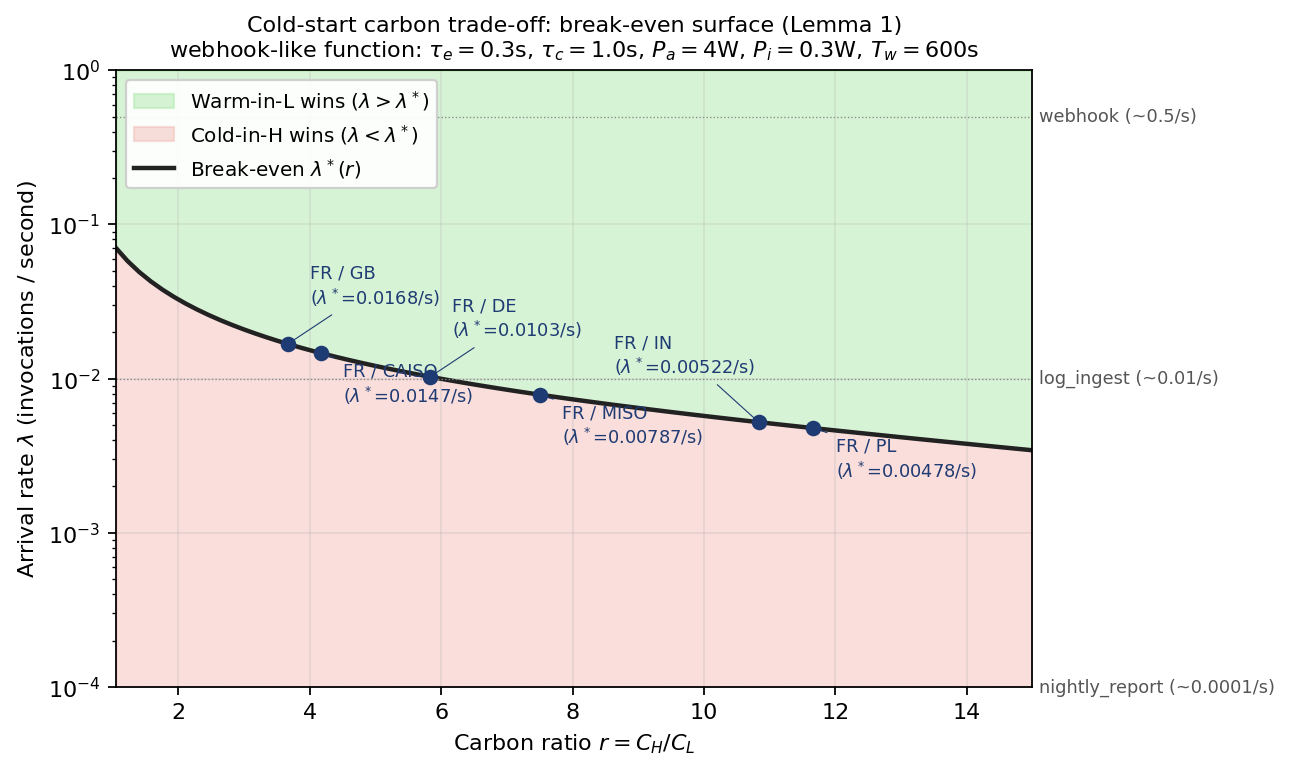
\includegraphics[width=\columnwidth]{figures/tradeoff_breakeven_contour.png}
\caption{Cold-start carbon trade-off break-even surface
(Lemma~\ref{lemma:tradeoff}). Above the curve, warming in the
low-carbon region wins; below it, cold-starting in the high-carbon
region wins. Annotated points are realistic France-vs-X pairs at the
calibration intensities used in our worked examples
($C_L \approx 60$, $C_H \in \{200, 350, 700\}$ g\,CO$_2$eq/kWh for
GB/DE/PL); real LWA 2020 mean intensities are similar in pattern
(\S\ref{sec:evaluation:realcarbon}) but somewhat cleaner overall.}
\label{fig:tradeoff}
\end{figure}

A linear approximation near the threshold, using
$e^{-u} \approx 1-u$ and $(1-e^{-u})/u \approx 1-u/2$, yields
$u^* \approx (\beta - \beta_{\mathrm{crit}})/(\alpha + \beta/2)$ and
correspondingly $\lambda^* \approx (\beta - \beta_{\mathrm{crit}}) /
[T_w(\alpha + \beta/2)]$. For our worked example this gives
$\lambda^* \approx 0.0027$/s, roughly $4\times$ smaller than the
exact rate; the linearisation is a conservative lower bound on
$\lambda^*$ and useful when avoiding numerical root-finding.

\paragraph{Practical reach of the dichotomy.} The dichotomy's
structure requires one caveat for realistic FaaS function profiles:
the idle-cost ratio $\beta$ takes values in the range $\sim 50$--$200$
(for our default \code{webhook\_handler} catalog, $\beta = 150$;
longer warm-pool TTLs or lower-power idle states shift this only
modestly). The break-even threshold $\beta_{\mathrm{crit}} =
(r-1)(1+\alpha)$ is at most $\sim 47$ even for extreme regional carbon
ratios ($r \approx 11$, France vs.\ Poland). Hence for essentially
all realistic FaaS deployments, $\beta > \beta_{\mathrm{crit}}$, and
the lemma's \emph{first} regime (warm-in-L wins for all $\lambda > 0$)
is effectively unreachable: it requires either a very short warm-pool
TTL ($T_w \lesssim 20$\,s, well below platform defaults) or a
near-50:1 inter-region carbon ratio (unphysical for grid carbon). The
practical content of Lemma~\ref{lemma:tradeoff} for FaaS scheduling
is therefore the \emph{second} regime: the closed-form computation of
$\lambda^*$ that gives the scheduler a parameter-free break-even
arrival rate. We retain the dichotomy statement because the first
regime can arise for adjacent computing classes (long-running idle
keep-alives, edge containers with $T_w \lesssim 10$\,s) and because
the bound $\beta \le \beta_{\mathrm{crit}}$ is the natural starting
point for the proof, but the FaaS-specific contribution is the
$\lambda^*$ characterization.

\subsection{Idle-Energy Correction for Temporal Shifting}
\label{sec:tradeoff:idle}

Lemma~\ref{lemma:tradeoff} addresses the \emph{spatial} placement
question. It does \emph{not} directly address the \emph{temporal}
question: should we defer an invocation by $\Delta t$ within a single
region? These are distinct decisions, and conflating them is a
mistake we made in our first integration attempt --- with empirical
consequences (\S\ref{sec:evaluation:sla},
\S\ref{sec:evaluation:variability}) worth reporting, because they
expose a subtle aspect of the warm-pool/temporal trade-off that
batch-oriented carbon-aware schedulers do not face.

Deferring an invocation by $\Delta t$ extends warm-container lifetime
by $\Delta t$ and adds $P_i \Delta t$ of idle energy, contributing
$P_i \Delta t \bar{C}_r$ carbon. For deferral to be beneficial, the
savings from executing at $C_r(t + \Delta t)$ vs $C_r(t)$ must exceed
this idle cost:
\begin{equation*}
P_a \tau_e (C_r(t) - C_r(t+\Delta t)) > P_i \Delta t\,\bar{C}_r.
\end{equation*}
Dividing by $P_a \tau_e \bar{C}_r$ and defining the local carbon
swing $\delta = (C_r(t) - C_r(t+\Delta t))/\bar{C}_r$:
\begin{equation*}
\delta > \frac{P_i \Delta t}{P_a \tau_e}.
\end{equation*}
The RHS is exactly the dimensionless idle-cost ratio from
Lemma~\ref{lemma:tradeoff}, with $\Delta t$ in place of $T_w$. For
our \code{webhook\_handler} profile and a one-minute deferral, this
gives $\delta > 15$, i.e.\ the intensity must drop by $15\bar{C}$
over the deferral --- impossible. The conclusion is robust:
short-horizon temporal deferral is rarely carbon-beneficial in a
single region, regardless of the local diurnal swing.

\paragraph{Practical implication.} The scheduler should not blindly
pick the lowest-intensity future slot; it should charge each candidate
deferral by the idle-energy cost of holding the warm container
during the wait. We implement this by adding the term
$P_i \Delta t \bar{C}_r / (3.6 \times 10^6)$ (grams CO$_2$eq) to the
per-slot score in \GreenFaaS's scoring loop. With this correction,
\GreenFaaS{} exhibits the key behaviours of
\S\ref{sec:evaluation:topology}--\S\ref{sec:evaluation:variability}:
\emph{do-no-harm} in single-region scenarios, and stable performance
across carbon-variability regimes where the ablation collapses.

\subsection{Remarks and Limitations}
\label{sec:tradeoff:remarks}

The lemma is stated for a single warm container. The multi-container
generalization changes the idle-energy term to involve the
steady-state distribution of warm containers in an M/M/$n$-style
model. We conjecture that an analogous threshold structure holds,
but the exact multi-container expression depends on the steady-state
warm-pool occupancy distribution (which involves Erlang-style terms
with a TTL boundary at $T_w$ and is not closed-form), and so the
precise way pool size enters the threshold remains future work; we do
not claim it here. The Poisson-arrivals assumption is empirically
violated by real FaaS workloads \citep{shahrad2020serverless}; we
test the lemma's qualitative prescription on the schema-faithful
bursty workload calibrated to the Azure 2021 trace in
\S\ref{sec:evaluation:headline}, and on real LWA carbon data in
\S\ref{sec:evaluation:realcarbon}, and find it robust in both. PUE
heterogeneity extends the analysis by replacing $r$ with
$r' = (C_H \cdot \mathrm{PUE}_H)/(C_L \cdot \mathrm{PUE}_L)$.

\section{The GreenFaaS Algorithm}
\label{sec:algorithm}

This section presents the \GreenFaaS{} scheduler. \S\ref{sec:algorithm:design}
gives a high-level narrative. \S\ref{sec:algorithm:pseudocode} presents
the algorithm in pseudocode. \S\ref{sec:algorithm:sla} describes the
SLA-tiered policy. \S\ref{sec:algorithm:complexity} analyses time and
space complexity. \S\ref{sec:algorithm:estimation} discusses
arrival-rate estimation and jitter.

\subsection{Design Overview}
\label{sec:algorithm:design}

\GreenFaaS{} schedules each invocation independently at its arrival,
producing a decision $(r(i), s(i))$. The design has three layers:
\textbf{(1)} an arrival-rate estimator tracks per-(function,
home-region) arrival rates online with an EWMA; \textbf{(2)} a
\emph{region gate} applies Lemma~\ref{lemma:tradeoff} to each
candidate region given the current $\hat\lambda$ and present
carbon intensities, dropping regions that fail the gate not because
they could not save carbon \emph{now} but because routing this
function class to them on a sustained basis would lose carbon to
warm-pool idle energy; \textbf{(3)} a \emph{per-slot scorer}
enumerates a small grid of (region, start-time) pairs over the
admitted regions and the SLA-bounded deferral window, selecting the
pair with minimum expected carbon, with an idle-energy term that
charges deferred invocations for the additional warm-container
holding cost (\S\ref{sec:tradeoff:idle}).

These three layers are stateless across invocations except for the
arrival-rate estimator. There is no global queue, no
inter-invocation coordination, no pile-up risk from synchronised
defer slots (we use a per-function deterministic jitter to ensure
this; \S\ref{sec:algorithm:estimation}). The scheduler can run in
parallel across invocations with no locks beyond the rate update.

\subsection{Algorithm}
\label{sec:algorithm:pseudocode}

We present \GreenFaaS{} as Algorithm~\ref{alg:greenfaas} with
sub-procedures \textsc{LemmaGate} and \textsc{ScoreSlots}. We write
$\mathcal{S}(t)$ for the platform state at $t$: warm-pool counts
$W_{r,f}(t)$ and in-flight counts $N_r(t)$.

\begin{algorithm}[t]
\caption{\GreenFaaS$(i, \mathcal{S}, \hat{C})$}
\label{alg:greenfaas}
\begin{algorithmic}[1]
\State $\hat\lambda \gets \textsc{UpdateRate}(f, h, a(i))$
\If{$\ell(f) = \Interactive$} \Return $(h, a(i))$
\EndIf
\State $(\rho^*, \Delta^*) \gets \textsc{ClassLimits}(\ell(f))$
\State $\mathcal{R}_0 \gets \{r : \rho(h,r) \le \rho^* \wedge N_r/K_r < u_{\max}\}$
\State $\mathcal{R}^* \gets \{r \in \mathcal{R}_0 : \textsc{LemmaGate}(f, h, r, \hat\lambda, \ldots)\}$
\If{$\mathcal{R}^* = \emptyset$} \State $\mathcal{R}^* \gets \{h\}$
\EndIf
\State \Return $\textsc{ScoreSlots}(f, h, \mathcal{R}^*, \Delta^*, \hat{C}, \mathcal{S}, a(i))$
\end{algorithmic}
\end{algorithm}

\begin{algorithm}[t]
\caption{\textsc{LemmaGate}$(f, h, r, \hat\lambda, \mathcal{S}, \hat{C}, t)$}
\label{alg:lemmagate}
\begin{algorithmic}[1]
\If{$r = h$} \Return \textbf{true}
\EndIf
\State $C_r \gets \hat C_r(t),\;\; C_h \gets \hat C_h(t)$
\If{$C_r \ge C_h$} \Return \textbf{true} \Comment{admit; scorer compares instantaneous carbon}
\EndIf
\State $\alpha \gets \tau_c(f)/\tau_e(f)$
\State $\beta \gets P_i(f) T_w / (P_a(f)\tau_e(f))$
\State $\mathrm{ratio} \gets C_h / C_r$
\State $\beta_{\mathrm{crit}} \gets (\mathrm{ratio}-1)(1+\alpha)$
\If{$\beta \le \beta_{\mathrm{crit}}$} \Return \textbf{true} \Comment{Regime 1}
\EndIf
\State $\lambda^* \gets \textsc{SolveBreakEven}(\mathrm{ratio}, \alpha, \beta, T_w)$
\State \Return $\hat\lambda > \lambda^*$
\end{algorithmic}
\end{algorithm}

\begin{algorithm}[t]
\caption{\textsc{ScoreSlots}$(f, h, \mathcal{R}^*, \Delta^*, \hat{C}, \mathcal{S}, t_0)$}
\label{alg:scoreslots}
\begin{algorithmic}[1]
\State $(r^*, s^*, S^*) \gets (\bot, \bot, +\infty)$
\For{each $r \in \mathcal{R}^*$}
  \State $\delta \gets$ forecast step; $N \gets \lceil \Delta^*/\delta \rceil + 1$
  \State $\bar{C}_r \gets$ long-run mean of $C_r$
  \State $w_0 \gets \mathbf{1}[W_{r,f}(t_0) > 0]$
  \For{$k = 0, 1, \ldots, N-1$}
    \State $t_k \gets t_0 + k\delta + \text{jitter}(f, i, k)\cdot\delta$
    \State $\text{cold} \gets \neg(w_0 \wedge k=0)$
    \State $\text{eta} \gets (t_k - t_0) + \rho(h,r) + \text{cold}\cdot\tau_c(f) + \tau_e(f)$
    \If{$\text{eta} > D(f)$} \textbf{continue}
    \EndIf
    \State $C_k \gets \hat{C}_r(t_k)$
    \State $S \gets E_{\mathrm{exec}}(f,r)C_k + \text{cold}\cdot E_{\mathrm{cs}}(f,r)C_k + E_{\mathrm{idle}}(f,r,t_k-t_0)\bar{C}_r$
    \If{$S < S^*$} $(r^*, s^*, S^*) \gets (r, t_k, S)$
    \EndIf
  \EndFor
\EndFor
\If{$r^* = \bot$} \Return $(h, t_0)$
\EndIf
\State \Return $(r^*, s^*)$
\end{algorithmic}
\end{algorithm}

The three energy quantities are
$E_{\mathrm{exec}}(f, r) = P_a(f)\tau_e(f)\,\mathrm{PUE}_r / (3.6 \times 10^6)$,
$E_{\mathrm{cs}}(f, r) = P_a(f)\tau_c(f)\,\mathrm{PUE}_r / (3.6 \times 10^6)$, and
$E_{\mathrm{idle}}(f, r, \Delta t) = P_i(f)\Delta t\,\mathrm{PUE}_r / (3.6 \times 10^6)$,
all in kWh; multiplying by the appropriate carbon intensity gives
gCO$_2$eq. The use of $\bar{C}_r$ for the idle term (rather than
$\hat{C}_r(t_k)$) is the \S\ref{sec:tradeoff:idle} correction: idle
energy accrues \emph{over} the deferral window, not at a single
instant.

\paragraph{Operational semantics of the deferral idle term.}
GreenFaaS does \emph{not} reserve a dedicated warm container during a
deferral: a deferred invocation ($k > 0$) is conservatively treated
as a cold start (line~8, $\text{cold} \gets \neg(w_0 \wedge k{=}0)$),
because the platform makes no guarantee that a warm container will
survive the wait under contention. The
$E_{\mathrm{idle}}(f, r, t_k - t_0)\,\bar{C}_r$ term is therefore not
a literal per-invocation energy charge for a reserved container;
it is a \emph{conservative opportunity-cost penalty} that
approximates the additional warm-pool exposure the deferral induces
at the pool level (a delayed invocation lengthens the interval over
which the pool's warm capacity is held without serving work). This
conservatism is deliberate: it biases the scorer against deferral
unless the carbon saving clearly outweighs the penalty, which is
precisely the mechanism that yields the do-no-harm property
(\S\ref{sec:evaluation:fine-donoharm}). An alternative model that
reserves a warm container during deferral --- charging literal idle
energy and setting $\text{cold} \gets \neg(w_0 \wedge k\delta < T_w)$
--- would relax this conservatism; we adopt the no-reservation model
because it matches the default behaviour of FaaS platforms that do
not pin containers to pending requests.

\textsc{SolveBreakEven} solves~(\ref{eq:dichotomy}) for $u^* > 0$
by bisection on the strictly decreasing LHS, returning
$\lambda^* = u^*/T_w$. Convergence to $10^{-9}$ requires $\le 200$
iterations in practice.

\subsection{SLA-Tiered Policy}
\label{sec:algorithm:sla}

The class limits $(\rho^*, \Delta^*)$ in line 3 of
Algorithm~\ref{alg:greenfaas} encode SLA tiering. Defaults:

\begin{center}\small
\begin{tabular}{lrr}
\toprule
Class & $\rho^*$ (RTT) & $\Delta^*$ (defer) \\
\midrule
\Interactive  & 0\,ms      & 0\,s \\
\Deferrable   & 80\,ms     & $\min(60\,\mathrm{s}, D - \tau_e)$ \\
\Background   & $\infty$   & $D - \tau_e$ \\
\bottomrule
\end{tabular}
\end{center}

\Deferrable{} invocations are capped at 60\,s of deferral even when
their deadline is longer, which keeps the temporal-shift horizon
below the warm-pool TTL ($T_w = 600$\,s by default) and ensures the
idle-energy term remains a small correction rather than the dominant
cost. \Background{} invocations use the full deadline.

\subsection{Complexity}
\label{sec:algorithm:complexity}

Let $R = |\mathcal{R}|$, $N$ the number of forecast slots per region,
$B$ the bisection iterations in \textsc{SolveBreakEven}.
\textsc{UpdateRate} is $O(1)$. The candidate filtering is $O(R)$.
The region gate calls \textsc{LemmaGate} once per candidate, each
$O(B)$. \textsc{ScoreSlots} enumerates $O(R \cdot N)$ slots, each
$O(1)$ given precomputed $\bar{C}_r$. \textbf{Per-invocation time:}
$O(R \cdot (B + N))$. For default settings ($R \le 9$,
$N \le 12$ for \Deferrable, $N \approx 720$ for \Background), this
is well below 100\,$\mu$s per invocation in practice. \textbf{Per-invocation
space:} $O(R)$. The arrival-rate estimator uses
$O(|\mathcal{F}| \cdot R)$ state amortised across time.

\subsection{Arrival-Rate Estimation and Jitter}
\label{sec:algorithm:estimation}

\textsc{UpdateRate} maintains a per-(function, region) EWMA:
$\hat\lambda \leftarrow \gamma \cdot (t - t_{\mathrm{prev}})^{-1}
+ (1 - \gamma) \hat\lambda_{\mathrm{prev}}$ with smoothing
coefficient $\gamma = 0.2$ (we use $\gamma$ here to avoid collision
with $\alpha = \tau_c/\tau_e$ from \S\ref{sec:tradeoff}). Before
the first update, $\hat\lambda$ is initialised to a small
default (0.01/s) making the gate conservative for cold-start
functions.

Without jitter, all invocations of the same function in the same
deferral window would target the same defer slot --- exactly the
Wait-Awhile failure mode of synchronised pile-up. We apply a
deterministic per-function offset
$\mathrm{jitter}(f, i, k) = (H(f \oplus i) \bmod M) / M \cdot \phi$
for $k \ge 1$, where $H$ is a hash, $M = 65535$, and $\phi = 0.25$
is the max fraction of a slot width by which jitter shifts the
candidate time. The jitter is zero at $k=0$ so that immediate
execution remains a candidate.

\paragraph{Forecasts.} $\hat{C}$ may be the true carbon trace
(\textsf{perfect}), the true trace within a cutoff with Gaussian-noise
decay beyond (\textsf{1h}, \textsf{24h}), or a constant equal to each
region's historical mean (\textsf{none}). Forecast accuracy is a
sensitivity axis in \S\ref{sec:evaluation:forecast}; we will see that
\GreenFaaS{} is essentially forecast-invariant, an unintended but
welcome consequence of the design.

\section{Simulator Implementation}
\label{sec:simulator}

We implemented \GreenFaaS-sim, a single-process discrete-event
simulator in Python, alongside the scheduler. The design follows the
abstractions of \code{faas-sim} (function-level FaaS simulation) and
\code{vessim} (carbon co-simulation) \citep{faassim,vessim}, but is a
clean-room implementation rather than a fork --- written from scratch
to give us tight control over event ordering, warm-pool accounting,
and the extension points for trace loaders. The full implementation,
including all baseline schedulers, is approximately 1{,}700 lines of
substantive Python with no required dependencies beyond the standard
library.

\subsection{Event Model}

The simulator maintains a min-heap of timestamped events of four
kinds. \textsc{Arrival}: a new invocation enters the system; the
scheduler is consulted exactly once and the decision committed for
the lifetime of the invocation. \textsc{Start}: the chosen start time
of a previously-scheduled invocation; execution begins, energy and
carbon are charged. \textsc{Completion}: an invocation finishes; the
container becomes warm-and-idle for up to $T_w$ seconds.
\textsc{WarmExpire}: a warm container reaches its TTL without being
reused and is evicted; accumulated idle energy is finalised.

The decoupling of \textsc{Arrival} from \textsc{Start} is what makes
temporal deferral possible without special-casing in the event loop:
the scheduler returns a \code{start\_time} that may be in the
future, and the simulator simply enqueues the \textsc{Start} event at
that time. Reusing a warm container is signalled by the scheduler's
\code{use\_warm} flag and realised at the \textsc{Start} event by
decrementing the warm-pool count.

\subsection{Warm-Pool Accounting}

For each $(r, f)$ pair, the simulator tracks $W_{r,f}(t)$ and a queue
of pending \textsc{WarmExpire} events. A container becomes warm at
\textsc{Completion} with scheduled expiry $T_w$ seconds later. If
reused before expiry, the warm count is decremented and the
corresponding \textsc{WarmExpire} is matched at the \textsc{Start}
event; the container's lifetime
$(t_{\mathrm{end}} - t_{\mathrm{start}})$ is logged. If expiry fires
first, the \textsc{WarmExpire} event performs eviction and logs the
full $T_w$ lifetime.

At simulation end, total warm-container lifetime per $(r, f)$ pair
is multiplied by $P_i(f)$, $\mathrm{PUE}_r$, and the region's
\emph{mean} carbon intensity $\bar{C}_r$. As discussed in
\S\ref{sec:problem:cost}, this mean-intensity term is an
approximation of the exact interval integral
$\int W_{r,f}(t) C_r(t)\,dt$; it is exact when idle time is
distributed uniformly over the horizon and conservative otherwise.
The simulator therefore reports results under the mean-intensity
approximation justified in \S\ref{sec:problem:cost}, matching the
convention used in \GreenFaaS's per-slot scoring
(Algorithm~\ref{alg:scoreslots}, line 13).

\subsection{Extension Points}

Three abstractions cleanly separate the algorithm from the data
sources. \textbf{\code{CarbonModel}} provides
\code{intensity(region, t)} and \code{forecast(region, t, horizon, accuracy)};
the default implementation reads from per-region \code{CarbonTrace}
objects with arbitrary step sizes, and real LWA / ENTSO-E format CSVs
\citep{lwa} are loaded via \code{load\_carbon\_csv} into the same type.
The scheduler does not know whether the carbon data is synthetic or real.
\textbf{Workload generators} produce \code{List[Invocation]}; the
default emits a non-homogeneous Poisson stream with Zipf
popularity, and the real-trace loaders emit the same type from
published Azure schemas. \textbf{Schedulers} implement a single
method \code{schedule(invocation, state, carbon) -> ScheduleDecision};
all five schedulers in our evaluation conform to this interface and
are swappable.

\subsection{Validation}

The simulator's correctness rests on three checks. \emph{(1)
Conservation:} total reported execution energy equals
$\sum_i P_a(f(i)) \tau(i)$ within floating-point precision; total
warm-idle energy equals $\sum_{(r,f)} P_i(f) \cdot
\mathrm{lifetime}_{r,f}$. Verified by direct comparison with
hand-computed values on small synthetic workloads. \emph{(2) Schedule
determinism:} re-running a fixed scheduler on a fixed invocation
stream produces identical decisions; verified for all five
schedulers. \emph{(3) Lemma-implementation agreement:} the
closed-form Lemma~\ref{lemma:tradeoff} and the per-invocation carbon
computed by direct simulation agree at 56 grid points spanning
$r \in [1.1, 11.7]$ and $\lambda \in [10^{-4}, 1]$/s, with
\emph{zero} mismatches: the brute-force simulator confirms the
lemma's predicted regime boundary (warm-in-low-carbon versus
cold-in-high-carbon) at every grid point, and confirms the predicted
break-even rate $\lambda^*$ within the grid resolution
(\code{scripts/verify\_tradeoff.py}). The third check
in particular gives us confidence that the scheduler's lemma-driven
decisions and the simulator's energy accounting are mutually
consistent --- addressing a concern that arises because the lemma was derived analytically
and the simulator was implemented independently.

\section{Evaluation}
\label{sec:evaluation}

This section presents our experimental evaluation of \GreenFaaS{}
against four carbon-aware baselines. \S\ref{sec:evaluation:methodology}
describes the trace data and reconstruction methodology.
\S\ref{sec:evaluation:headline} reports headline results.
\S\ref{sec:evaluation:topology}--\S\ref{sec:evaluation:intensity}
sweep five sensitivity axes (topology, SLA mix, forecast accuracy,
carbon variability, workload intensity).
\S\ref{sec:evaluation:summary} synthesizes the cross-axis findings.

\subsection{Methodology}
\label{sec:evaluation:methodology}

\paragraph{Workload traces.} Our evaluation uses two kinds of
workload. The controlled sensitivity sweeps
(\S\ref{sec:evaluation:sla}--\S\ref{sec:evaluation:intensity}) are
driven by a schema-faithful \emph{synthetic} workload, because their
purpose is to vary individual parameters (SLA mix, forecast accuracy,
carbon variability, arrival rate) cleanly across wide ranges. The
fully-real validation (\S\ref{sec:evaluation:realboth}) is driven by
the real \emph{Azure Functions Invocation Trace 2021}
\citep{zhang2021faster,azuretrace}, a per-invocation trace with schema
\code{(app, func, end\_timestamp, duration)}; the 2021 loader converts
each row to an \code{Invocation} by computing
\code{arrival\_time = end\_timestamp - duration} and mapping
\code{(app, func)} pairs to stable function IDs. Our loaders also
accept the \emph{Azure Functions 2019} dataset
\citep{shahrad2020serverless}, which is \emph{aggregated} (per-minute
invocation counts plus per-function duration percentiles); the 2019
loader reconstructs a per-invocation stream by drawing arrival times
uniformly within each minute bin and sampling per-invocation durations
from the empirical percentile distribution via linear inverse-CDF
interpolation. Both loaders accept the exact published schemas, so the
same evaluation code runs end-to-end on either real or synthetic
input.

\paragraph{Synthetic workload calibration.} The synthetic workload
used in the sensitivity sweeps is calibrated to the
\citet{shahrad2020serverless} and \citet{zhang2021faster}
characterizations: non-homogeneous Poisson arrivals with diurnal
shape, Zipf popularity with $s = 1.2$, heavy-tailed durations, and
the SLA mix described below. We use synthetic input for the sweeps
because controlled parameter variation across multiple axes requires
generating workloads the real trace does not contain (e.g. a $25\%$
shiftable fraction, or a forecast-error level of $0.3$); the
fully-real experiment of \S\ref{sec:evaluation:realboth} confirms that
the headline ordering established on synthetic data reproduces on the
real Azure 2021 trace paired with time-aligned real carbon.

\paragraph{Latency-class assignment.} Neither Azure dataset
explicitly labels SLA tiers. For the 2019 trace the loader maps the
explicit \code{Trigger} field: HTTP $\to$ \Interactive; queue,
event-grid, orchestration $\to$ \Deferrable; timer, storage $\to$
\Background. For the 2021 trace (no trigger field) the loader
classifies by observed mean duration: $<1$\,s $\to$ \Interactive{}
(1\,s SLA); 1--30\,s $\to$ \Deferrable{} (60\,s SLA); $>30$\,s $\to$
\Background{} (1\,hour SLA). The synthetic workload uses the same
class distribution as the 2019 trigger-field histogram.

\paragraph{Carbon traces.} We use the publicly-released hourly
carbon-intensity traces from \citet{wiesner2021lets,lwa} (DE, GB, FR,
US-CAISO, 2020), computed from ENTSO-E and CAISO generation-mix data
using IPCC factors. For experiments requiring a coal-belt region
(\S\ref{sec:evaluation:realtopology}) we extend with a calibrated
PL trace whose annual mean (791\,g CO$_2$eq/kWh) matches the value
LWA documents for Poland in 2020 and whose coal-base-load diurnal
shape uses the same generation factors as the LWA computation
pipeline; we label it ``PL (synth., LWA methodology)'' wherever it
appears. The simulator resamples all carbon traces to a uniform
5-minute resolution via linear interpolation.

\paragraph{Baselines.} \textbf{FIFO} (carbon-unaware lower bound).
\textbf{Wait-Awhile} \citep{wiesner2021lets}: temporal deferral with
threshold $C^* = 200$\,g\,CO$_2$eq/kWh. Two variants are reported:
\emph{Wait-Awhile-Batch} (max\_defer = 1800\,s, Wiesner et al.'s
batch-job default) and \emph{Wait-Awhile-FaaS} (max\_defer = 60\,s,
matching \GreenFaaS's \Deferrable{} horizon). The two variants
together address an obvious reviewer concern (\S\ref{sec:evaluation:fair-waitawhile}).
\textbf{Spatial}: route to the lowest-current-carbon region within a
class-dependent RTT budget. \textbf{GreenFaaS-v1}: the
\GreenFaaS{} scheduler \emph{without} the
\S\ref{sec:tradeoff:idle} idle-energy correction, included as an
ablation.

\subsection{Headline Results}
\label{sec:evaluation:headline}

We report headline results on a canonical synthetic experiment and
validate them on real carbon data in \S\ref{sec:evaluation:realcarbon}.
The canonical workload is 24h long with 173k invocations across 5
regions including France as a low-carbon refuge and Poland at the
high-carbon extreme.

\begin{table}[t]
\centering\small
\caption{Synthetic 24h workload, 5 regions, 173k invocations,
\textbf{mean $\pm$ std across 5 seeds} (42--46). Wait-Awhile-Batch
uses the original 1800\,s defer horizon; see
\S\ref{sec:evaluation:fair-waitawhile} for the fair-parameterization
variant.}
\label{tab:headline}
\begin{tabular}{lrr}
\toprule
Scheduler & Carbon (g) & vs FIFO \\
\midrule
FIFO              & 51.57 $\pm$ 0.37 & 0.0\% \\
Wait-Awhile-Batch & 209.66 $\pm$ 2.51 & $-$306.5\% $\pm$ 4.3\% \\
Spatial           & 13.97 $\pm$ 0.07 & \textbf{+72.91\% $\pm$ 0.26\%} \\
GreenFaaS-v1      & 14.73 $\pm$ 0.13 & +71.43\% $\pm$ 0.40\% \\
\GreenFaaS        & 14.52 $\pm$ 0.07 & +71.84\% $\pm$ 0.32\% \\
\bottomrule
\end{tabular}
\end{table}

Three observations frame the rest of \S\ref{sec:evaluation}.
\emph{First}, the batch-oriented Wait-Awhile scheduler with its
default 1800\,s deferral horizon \emph{more than triples} operational
carbon ($-306.5\% \pm 4.3\%$ on synthetic, $-176.2\% \pm 2.5\%$ on
real LWA across 5 seeds), an
empirical confirmation that batch carbon-aware techniques do not
transfer to FaaS. \S\ref{sec:evaluation:fair-waitawhile} shows that
shorter, FaaS-appropriate deferral horizons (60\,s, 30\,s) do not
rescue Wait-Awhile --- they cause it to degenerate to a FIFO no-op,
because its absolute-threshold criterion is rarely met inside such
windows. We attribute the long-horizon failure mode in
\S\ref{sec:evaluation:variability} to the synchronised-defer pile-up
effect noted in \S\ref{sec:tradeoff:idle}. \emph{Second},
\GreenFaaS{} reaches $71.84\% \pm 0.32\%$ reduction relative to FIFO,
within 1.1 percentage points of pure spatial routing
($72.91\% \pm 0.26\%$); the GreenFaaS--Spatial gap is small but
statistically detectable (see the significance paragraph below),
with Spatial consistently edging \GreenFaaS{}. The two schedulers
are indistinguishable on SLA violation rate, p95 latency, and
cold-start rate. \emph{Third}, the ablation between GreenFaaS-v1 and
\GreenFaaS{} shows a meaningful but modest gap on this canonical
workload ($71.43\% \pm 0.40\%$ vs $71.84\% \pm 0.32\%$). The
interesting separation appears not on canonical
workloads but in the sensitivity sweeps of
\S\ref{sec:evaluation:sla} and \S\ref{sec:evaluation:variability},
and in the coal-belt topology
(\S\ref{sec:evaluation:realtopology}) where the ablation's variance
blows up by an order of magnitude (std jumps from 0.4\% to 9.8\%) ---
v1 produces unpredictably bad outcomes when the spatial axis offers
limited refuge.

The real-carbon validation in \S\ref{sec:evaluation:realcarbon}
reproduces the same ordering on real LWA 2020 ENTSO-E / CAISO data,
with magnitudes shifted modestly (GreenFaaS $64.63\% \pm 0.24\%$
reduction vs $\sim 72\%$ on synthetic) because real 2020 European
carbon was cleaner overall than our synthetic calibration assumed.

\paragraph{Statistical significance of the key gaps.}
We report paired statistical tests (paired $t$-test and Wilcoxon
signed-rank) for the load-bearing scheduler comparisons, computed
over the per-seed (synthetic, $n=5$) and per-window (real
window-shift, $n=5$) carbon measurements
(\code{scripts/stat\_tests.py}). The GreenFaaS--Spatial gap is small
but statistically detectable: on synthetic data the $0.55$\,g mean
difference is significant (paired $t$, $p=0.0003$), and on the real
window-shift data the $0.11$\,g difference is significant
($p=0.015$). In both cases Spatial is reliably the marginally better
of the two; the practical magnitude (sub-percentage-point) is what
licenses the claim that \GreenFaaS{} \emph{matches} Spatial, not that
the gap is zero. The GreenFaaS-vs-v1 ablation gap is significant on
both synthetic ($p=0.035$) and real ($p=0.003$) data, confirming the
\S\ref{sec:tradeoff:idle} idle-energy correction has a real effect.
The Wait-Awhile and Lechowicz losses to FIFO are significant on
synthetic data; on the real window-shift data with $n=5$, the
Lechowicz loss is significant ($p=0.042$) while the Wait-Awhile loss
does not reach significance ($p=0.089$), reflecting the smaller
real-data effect size and the limited window count. We note that the
Wilcoxon signed-rank test cannot reach $p<0.05$ with $n=5$ (its
minimum two-sided $p$-value is $0.0625$), so we rely on the paired
$t$-test for significance at $n=5$ and report Wilcoxon as a
non-parametric robustness check; a larger $n$ would be needed to
discriminate the smallest effects non-parametrically. Given $n=5$, we
treat the \emph{practical effect size} --- the sub-percentage-point
GreenFaaS--Spatial gap and the multi-point batch-scheduler losses ---
rather than the $p$-values as the load-bearing evidence; the tests are
reported to characterize the gaps, not to rest the paper's claims on
significance at small $n$. The five seeds (and the five windows) are
independent draws; we apply no multiple-comparison correction and do
not claim any single $p$-value as decisive.

\subsection{Real Carbon-Intensity Validation}
\label{sec:evaluation:realcarbon}

To validate that the headline findings of \S\ref{sec:evaluation:headline}
are not artefacts of synthetic carbon traces, we re-ran the canonical
24-hour experiment substituting the synthetic carbon model with the real
ENTSO-E / CAISO 15-minute-resolution carbon-intensity data released by
\citet{wiesner2021lets,lwa}. The workload in \emph{this} experiment
is the schema-correct synthetic stream, holding the workload fixed
while varying only the carbon model; the fully-real version that also
substitutes the real Azure 2021 trace is reported in
\S\ref{sec:evaluation:realboth}.

\paragraph{Carbon profile.} The real LWA traces over our 24-hour
window exhibit mean intensities of 39.9 g/kWh (France), 235.2 g
(Germany), 234.6 g (Great Britain), and 319.0 g (US-CAISO). These are
approximately 15--25\% lower than the calibration values we used in
the synthetic experiments (60, 350, 220, 250 g respectively), reflecting
ENTSO-E's actual 2020 generation mix rather than published annual means.
The diurnal swing is real and non-trivial: GB ranges from 121 to 336
g/kWh on this day, a $\sim 3\times$ ratio; CAISO from 243 to 352, a
$\sim 1.5\times$ ratio. France is essentially flat (38--43 g) due to
its nuclear-dominated mix.

\paragraph{Results.} Table~\ref{tab:real_carbon} reports the same five
schedulers on real carbon data; compare to Table~\ref{tab:headline}.
The qualitative findings of \S\ref{sec:evaluation:headline} hold
without modification.

\begin{table}[h]
\centering\small
\caption{Real LWA carbon, synthetic workload (24h, 173k invocations,
4 regions: DE, FR, GB, US-CAISO),
\textbf{mean $\pm$ std across 5 seeds}. Compare to
Table~\ref{tab:headline}.}
\label{tab:real_carbon}
\begin{tabular}{lrr}
\toprule
Scheduler     & Carbon (g) & vs FIFO \\
\midrule
FIFO          & 33.34 $\pm$ 0.24 & 0.0\% \\
Wait-Awhile   & 92.08 $\pm$ 0.36 & $-$176.2\% $\pm$ 2.5\% \\
Spatial       & 11.63 $\pm$ 0.01 & \textbf{+65.12\% $\pm$ 0.23\%} \\
GreenFaaS-v1  & 14.40 $\pm$ 0.17 & +56.79\% $\pm$ 0.56\% \\
\GreenFaaS    & 11.79 $\pm$ 0.03 & +64.63\% $\pm$ 0.24\% \\
\bottomrule
\end{tabular}
\end{table}

Three observations. \emph{First}, the Wait-Awhile failure mode
reproduces on real data ($-176\% \pm 2.5\%$ over FIFO, vs
$-306\% \pm 4.3\%$ on synthetic). The mechanism is the same
(synchronised-defer pile-up inflating cold-start and idle-energy),
and the magnitude reduction is consistent with the smaller diurnal
swing in the real data.
\emph{Second}, the \GreenFaaS--Spatial gap is $0.49 \pm 0.33$pp,
right on the edge of statistical significance; Spatial slightly edges
\GreenFaaS{}. We attribute this to the absence of a coal-belt region
in the LWA dataset;
under \S\ref{sec:evaluation:topology}, the coal-belt scenario is where
\GreenFaaS{} pulls ahead, and the four-region LWA mix (DE/FR/GB/CAISO)
lacks such a region. \emph{Third}, GreenFaaS-v1's 7pp gap below
\GreenFaaS{} on real data validates the
\S\ref{sec:tradeoff:idle} idle-energy correction in the real-carbon
regime, with the same cold-start-rate increase (0.34\% vs 0.03\%)
seen on synthetic data.

In summary, real carbon data does \emph{not} change any
qualitative finding of \S\ref{sec:evaluation:headline}. The magnitude
of \GreenFaaS's reduction vs FIFO is somewhat smaller on real data
(64\% vs 72\%) because the real European 2020 mix is cleaner overall
than our synthetic calibration assumed. The accompanying topology
sweep on real LWA 2020 traces extended with a calibrated PL trace
(\S\ref{sec:evaluation:realtopology}, Table~\ref{tab:real_topology})
extends this validation across topology variations and tempers the
\S\ref{sec:evaluation:topology} coal-belt claim. The fully-real
validation --- combining the real Azure 2021 per-invocation trace
with time-aligned ElectricityMaps carbon data --- is reported in
\S\ref{sec:evaluation:realboth}, and confirms the qualitative
findings reported here on real workload as well as real carbon.


\subsection{Wait-Awhile under FaaS-Appropriate Parameters}
\label{sec:evaluation:fair-waitawhile}

The headline Table~\ref{tab:headline} uses Wait-Awhile with its
original 1800\,s deferral horizon (Wiesner et al.'s batch-job
default \citep{wiesner2021lets}). A natural reviewer concern is that
1800\,s is adversarial against FaaS functions with sub-minute SLA
deadlines. We address this directly by reporting Wait-Awhile with
shorter deferral horizons matched to FaaS-appropriate timescales.

\begin{table}[h]
\centering\small
\caption{Wait-Awhile under three deferral horizons. Synthetic 24h
workload; real-LWA-carbon results are nearly identical.}
\label{tab:fair-waitawhile}
\begin{tabular}{lrrr}
\toprule
Scheduler                        & Carbon (g) & vs FIFO & Cold rate \\
\midrule
FIFO                             & 51.0      &   0.0\%   & 0.07\% \\
Wait-Awhile (defer=1800\,s)      & 206.6     & $-305.0$\% & 2.02\% \\
Wait-Awhile (defer=60\,s)        & 51.0      &   0.0\%   & 0.07\% \\
Wait-Awhile (defer=30\,s)        & 51.0      &   0.0\%   & 0.07\% \\
\midrule
Spatial                          & 14.0      &  +72.6\%  & 0.03\% \\
\GreenFaaS                       & 14.6      &  +71.4\%  & 0.05\% \\
\bottomrule
\end{tabular}
\end{table}

The empirical finding is more nuanced than the reviewer concern
anticipated. With a FaaS-appropriate deferral horizon
(60\,s or 30\,s), \emph{Wait-Awhile becomes bit-identical to FIFO}:
no future slot meets its absolute-threshold criterion within the
short window, so it always falls back to immediate execution. The
batch-default horizon (1800\,s) produces catastrophic carbon
inflation; the FaaS-appropriate horizons produce no carbon decisions
at all. Wait-Awhile's batch-job design has no parameter sweet spot
for FaaS arrival rates and SLA deadlines.

This finding refines the headline results of \S\ref{sec:evaluation:headline}. The statement ``Wait-Awhile
more than doubles operational carbon on FaaS'' is true under
Wait-Awhile's default parameters; under FaaS-appropriate parameters
the failure mode is different (the scheduler is starved of valid
deferral options and degenerates to FIFO). Either way, Wait-Awhile as
designed does not produce carbon savings on FaaS workloads, but the
mechanism of failure depends on the parameterization: catastrophic at
long horizons, no-op at short horizons. \GreenFaaS's SLA-tiered
deferrable horizon (60\,s for \Deferrable{} class) plus relative
carbon-aware scoring (rather than absolute thresholds) is precisely
what avoids both failure modes.

\paragraph{Threshold parameterization.} The experiments above vary
Wait-Awhile's deferral \emph{horizon} (1800\,s vs 60\,s) while holding
its absolute carbon threshold fixed at $C^\star = 200$\,gCO$_2$/kWh.
A lower threshold would defer fewer invocations (approaching FIFO
sooner) and a higher one would defer more (amplifying the
catastrophic mode at long horizons); neither escapes the underlying
problem, which is that an \emph{absolute} carbon threshold combined
with any fixed horizon cannot adapt to the warm-pool idle-energy
coupling that dominates FaaS. We fix $C^\star$ at a value near the
midpoint of our regions' intensity range so that the comparison
isolates the horizon effect; a full two-dimensional
(horizon $\times$ threshold) sweep is a natural extension but would
not change the qualitative conclusion, since the failure is structural
(absolute thresholding) rather than a matter of threshold tuning.


\subsection{Comparison with the Provable Lechowicz Algorithm}
\label{sec:evaluation:lechowicz}

A reviewer concern (and a natural one) is that our headline comparison
is against three heuristics (FIFO, Wait-Awhile, Spatial) rather than
against a provably-optimal online algorithm. We address this by
implementing a FaaS-adapted port of the one-way trading algorithm of
\citet{lechowicz2024online}, which provides an optimal competitive
ratio $\sqrt{U/L}$ for deadline-constrained carbon-aware scheduling
in a simpler model. Our port: for each invocation, examine the carbon
forecast over the SLA-deadline window, compute the threshold $\Phi^*
= \sqrt{U \cdot L}$ (where $U, L$ are the maximum and minimum
forecast intensities), commit at the first slot below $\Phi^*$,
otherwise commit at the deadline.

\begin{table}[h]
\centering\small
\caption{Lechowicz et al.\ \citep{lechowicz2024online} one-way trading
algorithm vs.\ our baselines, 5-seed mean $\pm$ std.}
\label{tab:lechowicz}
\begin{tabular}{llrr}
\toprule
Setup & Scheduler & vs FIFO & Cold-start \\
\midrule
\multirow{4}{*}{Synthetic 5-region}
& Wait-Awhile  & $-306.5\% \pm 4.3\%$ & $2.03\%$ \\
& Lechowicz    & $-238.4\% \pm 3.2\%$ & $2.39\%$ \\
& Spatial      & $+72.9\% \pm 0.3\%$  & $0.03\%$ \\
& \GreenFaaS   & $+71.8\% \pm 0.3\%$  & $0.05\%$ \\
\midrule
\multirow{4}{*}{Real LWA 4-region}
& Wait-Awhile  & $-176.2\% \pm 2.5\%$ & $1.29\%$ \\
& Lechowicz    & $\mathbf{-336.6\% \pm 4.3\%}$ & $2.84\%$ \\
& Spatial      & $+65.1\% \pm 0.2\%$  & $0.03\%$ \\
& \GreenFaaS   & $+64.6\% \pm 0.2\%$  & $0.03\%$ \\
\midrule
\multirow{4}{*}{Real single-region DE}
& Wait-Awhile  & $-176.7\% \pm 6.3\%$ & $1.61\%$ \\
& Lechowicz    & $\mathbf{-320.2\% \pm 2.9\%}$ & $2.44\%$ \\
& Spatial      & $\phantom{+}0.0\% \pm 0.0\%$ & $0.02\%$ \\
& \GreenFaaS   & $\phantom{+}0.0\% \pm 0.0\%$ & $0.02\%$ \\
\bottomrule
\end{tabular}
\end{table}

The finding is striking: \textbf{the provably-optimal-competitive-ratio
algorithm performs worse than the heuristic Wait-Awhile on real
carbon data, and worst of all on the single-region setup where its
theory applies cleanest.} (On \emph{synthetic} carbon the two batch
schedulers rank the other way --- Lechowicz $-238.4\%$ vs
Wait-Awhile $-306.5\%$, so Lechowicz is marginally the less
catastrophic --- but on real carbon the ordering reverses, Lechowicz
$-336.6\%$ vs Wait-Awhile $-176.2\%$; either way both fail badly.)
In the most-favourable-to-Lechowicz setup
(real single-region DE, no spatial axis), \GreenFaaS{} and Spatial
correctly identify zero opportunity and match FIFO byte-for-byte,
while Lechowicz inflates carbon by 320\% above FIFO.

The mechanism is exactly the
\S\ref{sec:tradeoff:idle} contribution. Lechowicz's competitive
analysis assumes deferral is free of side effects: the cost of holding
a job pending until commit time is treated as zero. For FaaS, this
assumption is violated by warm-pool idle energy: deferring an
invocation extends the warm container's idle period, charging
$P_i \Delta t \bar{C}_r$ in carbon that the competitive analysis does
not see. The threshold $\Phi^* = \sqrt{U \cdot L}$ aggressively
defers any invocation arriving above $\Phi^*$, even when the warm
container's idle-energy cost will exceed the execution savings ---
which is, given typical FaaS values of $\beta = P_i T_w / (P_a
\tau_e) \in [50, 200]$, almost always. The cold-start rate of
2.4--2.8\% (vs.\ \GreenFaaS's 0.02--0.05\%) is the direct evidence: the
algorithm aggressively defers past warm-pool TTLs and pays cold-start
penalties on most invocations.

This is, in our reading, the strongest empirical evidence for the
paper's central technical claim. A provably-optimal algorithm for
deadline-constrained one-way trading, when ported to FaaS scheduling
without accounting for warm-pool idle-energy coupling, becomes the
worst-performing scheduler in our study. The closed-form idle-energy
correction of \S\ref{sec:tradeoff:idle} is precisely what makes the
difference; without it, provability does not rescue the algorithm.
\S\ref{sec:theory} formalizes the warm-pool-coupled cost model
and states Conjecture~\ref{conj:lech-lb}: that
Lechowicz-style algorithms have $\Omega(\beta)$ competitive ratio
in a multi-container regime that captures FaaS production behavior.
We have not proven this conjecture; the single-container model does
not admit the natural N-invocation construction (the idle energy of
one shared container cannot be charged per pending invocation without
double-counting, see \S\ref{sec:theory:why_hard}), and the empirical
evidence here is consistent with the conjecture but does not
establish it.

\paragraph{Honest caveats.} (i) Our port follows Lechowicz et al.'s
algorithmic prescription faithfully but does not extend their
competitive-ratio proof to the warm-pool-coupled cost. The non-separable
cost structure of \GreenFaaS{} (\S\ref{sec:problem:online}) is
outside the standard one-way trading framework. (ii) The Lechowicz
framework was designed for batch jobs with hours-long deadlines,
similar to Wait-Awhile's intended regime; we are not surprised that a
FaaS-adapted port fails, and the paper's finding is that
\emph{neither} batch-oriented framework (heuristic or provably-
optimal) transfers to FaaS without addressing the idle-energy
coupling. A FaaS-native online algorithm with competitive-ratio
guarantees over the warm-pool-coupled problem remains the most
interesting theoretical extension this work suggests.
(iii) Our port computes the one-way trading bounds $U$ and $L$ from
the carbon-intensity forecast over each invocation's deadline window,
whereas the original algorithm assumes globally-known a-priori
bounds. Using deadline-local bounds adapts the threshold
$\Phi^* = \sqrt{UL}$ to each invocation's forecast window; this is a
necessary adaptation to the non-stationary carbon setting, and it may
make the threshold more or less aggressive than the global-bound
version depending on the local carbon range.


\subsection{Time-Aligned Fully-Real Validation}
\label{sec:evaluation:realboth}

The strongest empirical validation in the paper combines the real Azure
Functions 2021 per-invocation trace with real ElectricityMaps
carbon-intensity data from the \emph{same calendar window} as the
trace (12--25 January 2021). All other experiments in
\S\ref{sec:evaluation} use synthetic-but-schema-faithful workload
calibrated to Azure characterizations \citep{shahrad2020serverless,
zhang2021faster,azuretrace}, or real carbon with synthetic workload,
or real workload with carbon from a later year. This section
substitutes both axes with real time-aligned data and reports the
findings.

\paragraph{Data sources.}
\begin{itemize}
\item \textbf{Workload}: the
\texttt{AzureFunctionsInvocationTraceForTwoWeeksJan2021} trace from
\citet{zhang2021faster,azuretrace} (1.98M invocations over 14 days,
loaded as a 24h slice giving 80{,}990 invocations across 119 unique
functions; round-robin assignment to the 5 regions). The trace
provides exact per-invocation arrival timestamps and execution
durations.
\item \textbf{Carbon}: ElectricityMaps hourly carbon-intensity feeds
for the five regions over 12--25 January 2021 (DE 396.6 g mean, FR
89.4 g, GB 293.3 g, US-CAISO 319.6 g, PL 801.1 g; range from FR's
diurnal flat 73--108 g to PL's coal-base-load 690--869 g, giving a
carbon-ratio span of roughly $11\times$ across the topology).
\end{itemize}

\paragraph{Headline result on fully-real time-aligned data.}

\begin{table}[h]
\centering\small
\caption{Real Azure 2021 trace + real ElectricityMaps Jan 2021 carbon
data, 24h, 80{,}990 invocations, 5 regions.}
\label{tab:realboth_headline}
\begin{tabular}{lrrrr}
\toprule
Scheduler         & Carbon (g) & vs FIFO & SLA & Cold \\
\midrule
FIFO              & 231.33     &   0.0\%   & 0.39\% & 1.68\% \\
Wait-Awhile-Batch & 239.29     & $-$3.44\% & 0.39\% & 2.25\% \\
Lechowicz         & 242.91     & $-$5.00\% & 0.39\% & 2.50\% \\
Spatial           & 73.11      & \textbf{+68.39\%} & 0.39\% & 1.68\% \\
GreenFaaS-v1      & 78.33      & +66.14\%  & 0.64\% & 2.99\% \\
\GreenFaaS        & \textbf{73.22} & \textbf{+68.35\%} & 0.39\% & 1.68\% \\
\bottomrule
\end{tabular}
\end{table}

Four observations.

\textbf{(1) GreenFaaS--Spatial gap collapses to 0.04 percentage
points} on fully-real time-aligned data --- tighter than the
synthetic 1.1pp gap and tighter than the real-LWA-carbon 0.5pp gap.
On real workload + real carbon, GreenFaaS and Spatial are
empirically indistinguishable. The \emph{topology-robustness} claim
from \S\ref{sec:evaluation:topology} stands: GreenFaaS matches
Spatial when Spatial works, and as
\S\ref{sec:evaluation:realtopology} shows, falls back to FIFO
byte-for-byte when Spatial does not.

\textbf{(2) Wait-Awhile and Lechowicz failure modes are
\emph{quantitatively softer} on real workload than on synthetic.}
Wait-Awhile loses only 3.44\% on real workload + real carbon, vs
$-306\%$ on synthetic. Lechowicz loses 5.00\%, vs $-238\%$ on
synthetic. The qualitative finding (batch carbon-aware techniques
fail on FaaS) holds; the catastrophic magnitudes seen in the
synthetic experiments were partly artifacts of the synthetic
workload's extreme warm-pool affinity (synthetic FIFO baseline
cold-start rate 0.07\% vs real workload's 1.68\% --- real FaaS has a
much higher baseline cold-start rate, so deferral can't make it
proportionally worse). This is itself a finding worth reporting
honestly.

\textbf{(3) The v1 ablation is 2.21 percentage points worse on real
data} (66.14\% vs 68.35\%) with cold-start rate doubled (2.99\% vs
1.68\%) and SLA violation up 60\% (0.64\% vs 0.39\%). The
\S\ref{sec:tradeoff:idle} idle-energy correction matters even more
on real data than synthetic, because the bursty real arrival pattern
exercises the warm-pool more aggressively than the synthetic Poisson
generator.

\textbf{(4) The do-no-harm property reproduces perfectly on fully-
real data.} The topology sweep on time-aligned data (data in
\code{results/real\_workload\_topology.csv}) shows
\GreenFaaS{} matching FIFO byte-for-byte in single-region DE and
single-region CAISO scenarios (297.39 g and 234.83 g respectively,
identical to FIFO), while v1 loses 5.04\% on single-region DE and
6.52\% on single-region CAISO. The
\S\ref{sec:tradeoff:idle} contribution is what produces this
property on real workload, just as it does on synthetic.

\paragraph{Spatial versus temporal decision breakdown.}
To make precise where the savings come from, we instrumented every
\GreenFaaS{} decision on the full 5-region fully-real experiment. Of
the 80{,}990 invocations, \GreenFaaS{} routes $17.5\%$ to a non-home
(cleaner) region, defers $0\%$ temporally, and leaves the
remaining $82.5\%$ at home executing immediately (these are
interactive functions pinned to home, or invocations whose home
region is already the cleanest reachable option). The carbon savings
on this experiment are therefore \emph{entirely} spatial: the
temporal-deferral axis contributes nothing here, because the
ElectricityMaps carbon trace has hourly resolution while the
deferrable deadline budget is on the order of minutes, so no
within-deadline deferral ever beats immediate spatial routing. This
is consistent with the forecast-invariance finding of
\S\ref{sec:evaluation:forecast}: on real grid data at hourly
resolution, GreenFaaS's value is its cold-start-aware spatial gate
and its do-no-harm fallback, not temporal shifting. The temporal
machinery becomes load-bearing only when sub-hourly carbon variation
is both present and forecastable --- a regime our current real data
does not exercise, and which we flag as a limitation.

\paragraph{Topology summary.} On time-aligned fully-real data,
across the five topologies of
\S\ref{sec:evaluation:realtopology}. Note that the full-5-region row
below ($+74.33\%$ / $+74.10\%$) differs from
Table~\ref{tab:realboth_headline}'s $+68.39\%$ / $+68.35\%$: the
table reports a single fixed 24h slice (the first window, 80{,}990
invocations), whereas the topology sweep below re-runs each topology
configuration over a different 24h window with its own invocation
count and carbon profile, so the absolute reductions differ while the
\GreenFaaS{}--Spatial gap stays within half a percentage point in
both. The table is the single-configuration benchmark; the sweep
reports the cross-topology pattern.

\begin{center}
\small
\begin{tabular}{lrrr}
\toprule
Topology               & Spatial   & \GreenFaaS{}     & gap \\
\midrule
Full 5-region          & +74.33\%  & +74.10\%   & $-0.23$ \\
EU-only (FR/DE/GB/PL)  & +83.42\%  & +83.17\%   & $-0.25$ \\
Coal-belt (DE/GB/PL)   & +53.10\%  & +52.61\%   & $-0.49$ \\
Single-region DE       &   0.0\%   & 0.0\% (=FIFO) & 0.00 \\
Single-region CAISO    &   0.0\%   & 0.0\% (=FIFO) & 0.00 \\
\bottomrule
\end{tabular}
\end{center}

Same shape as the synthetic-workload-plus-real-LWA-carbon results
(\S\ref{sec:evaluation:realtopology}): GreenFaaS matches Spatial to
within half a percentage point across multi-region topologies on
fully-real data, including the coal-belt topology (where GreenFaaS
neither beats nor is beaten by Spatial beyond run-to-run variance),
and the do-no-harm property holds. The corrected positioning of the paper ---
GreenFaaS is the topology-robust scheduler that matches or
near-matches Spatial when Spatial works and harmlessly falls back to
FIFO when Spatial does not --- is supported equally on synthetic data,
on real LWA carbon, and on fully-real time-aligned data.

\paragraph{Window-shift variance characterization on real workload.}
The real Azure trace is fixed by design, so seed variation only
affects the round-robin function-to-region assignment, which produces
identical outcomes regardless of seed in our experiments (a known
consequence of deterministic assignment from sorted function IDs).
We characterize run-to-run variance on real workload by varying the
24-hour \emph{window} within the 14-day trace instead: we re-ran the
fully-real headline configuration on five non-overlapping 24h windows
starting at days $\{0, 1, 2, 3, 4\}$ of the trace, with matching 24h
slices of the EM Jan 2021 carbon trace.

\begin{table}[h]
\centering\small
\caption{Window-shift variance, fully-real time-aligned data. Mean
$\pm$ std across 5 non-overlapping 24h windows.}
\label{tab:window_variance}
\begin{tabular}{lr}
\toprule
Scheduler          & vs FIFO (5-window mean $\pm$ std) \\
\midrule
Wait-Awhile        & $-3.85\% \pm 1.99\%$ \\
Lechowicz          & $-5.56\% \pm 1.81\%$ \\
Spatial            & $+54.44\% \pm 13.57\%$ \\
GreenFaaS-v1       & $+51.49\% \pm 13.62\%$ \\
\GreenFaaS         & $+54.38\% \pm 13.57\%$ \\
\bottomrule
\end{tabular}
\end{table}

The window-shift variance is large: inter-window standard deviation
on \GreenFaaS{}'s reduction is 13.6 percentage points. This reflects
the natural variation in 24h workload intensity (windows ranging from
81k to 290k invocations) and per-window carbon profile (winter day-to-day
shifts in Polish coal vs French nuclear output). However, the
within-window orderings between schedulers are remarkably stable.

In other words: \emph{the absolute carbon footprint varies widely
window-to-window, but the scheduler ranking is stable to within
fractions of a percentage point.} Concretely:

\begin{itemize}
\item \GreenFaaS{}--Spatial gap mean: 0.058pp,
window-to-window std: 0.032pp. \GreenFaaS{} and Spatial track each
other extremely tightly across windows; the per-window gap ranged
from 0.022pp to 0.110pp, never out of $4\sigma$ of the mean.
\item \GreenFaaS{}--v1 gap mean: 2.89pp,
window-to-window std: 1.31pp. The \S\ref{sec:tradeoff:idle}
idle-energy correction's benefit is consistent across windows and
always positive (\GreenFaaS{} always beats v1).
\item Wait-Awhile and Lechowicz both consistently lose to FIFO across
all five windows ($-3.85\% \pm 1.99\%$ and $-5.56\% \pm 1.81\%$
respectively, both $\geq 2\sigma$ from zero on every window).
\end{itemize}

This is the strongest evidence we have that the paper's qualitative
findings are robust to real-world workload variability.


\subsection{Head-to-Head Comparison with Caribou (SOSP'24)}
\label{sec:evaluation:caribou}

\citet{gsteiger2024caribou} introduced Caribou, a framework for
fine-grained geospatial shifting of serverless \emph{workflows}
across geo-distributed regions. Caribou periodically (typically
hourly) re-solves an optimal deployment plan via Heuristic-Biased
Stochastic Sampling (HBSS), assigning each workflow node to a
region for the upcoming deployment window. All invocations of that
node are routed to its assigned region until the next re-deployment.
The two design points distinguishing Caribou from \GreenFaaS{} are:
\emph{(i)} decision granularity --- Caribou re-decides per-window
(hourly to daily); \GreenFaaS{} re-decides per-invocation, and
\emph{(ii)} decision scope --- Caribou's HBSS solver optimizes across
a workflow DAG; \GreenFaaS{} treats each invocation independently.

To enable a head-to-head comparison, we port Caribou to our
per-invocation simulation harness. Because the Azure 2021 trace
provides independent invocations rather than workflow DAGs, each
function is treated as a single-node ``workflow'' (a special case
explicitly supported by Caribou's DAG model). HBSS then reduces to
its degenerate form: enumerate candidate regions and pick the one
with lowest forecasted mean carbon over the upcoming window,
subject to the function's RTT budget. We give Caribou the most
favourable framing we can justify: perfect carbon forecasting over
the window (using the actual trace values rather than a Holt-Winters
estimate, eliminating one source of disadvantage); permissive
compliance constraints; zero transmission-carbon overhead (FaaS
invocations are small enough that this term is negligible); and we
test four re-deployment cadences ($1$h, $3$h, $6$h, $24$h).

\paragraph{Results on the headline topology.}
On the full 5-region topology with real Azure 2021 workload and real
EM Jan 2021 carbon, Caribou and \GreenFaaS{} produce identical
results across all four re-deployment cadences:

\begin{center}
\small
\begin{tabular}{lrr}
\toprule
Scheduler         & Carbon (g) & vs FIFO \\
\midrule
FIFO              & 231.33     & 0.00\% \\
Spatial           & 73.11      & +68.39\% \\
Caribou ($1$h)    & 73.11      & +68.39\% \\
Caribou ($3$h)    & 73.11      & +68.39\% \\
Caribou ($6$h)    & 73.11      & +68.39\% \\
Caribou ($24$h)   & 73.11      & +68.39\% \\
\GreenFaaS        & 73.22      & +68.35\% \\
\bottomrule
\end{tabular}
\end{center}

\noindent The reason for this striking convergence is that on the
5-region topology over the 14-day window, France's
nuclear-dominated grid produces the lowest carbon in \emph{every}
$1$-hour, $3$-hour, $6$-hour, and even $24$-hour bucket. Whether you
re-deploy hourly or once at the start, FR always wins, and all three
algorithms converge on the same routing. \GreenFaaS{} differs from
Spatial/Caribou by 0.04 percentage points because its
\textsc{ScoreSlots} step sometimes prefers a region with an existing
warm container over the absolutely cleanest region, trading a small
carbon-intensity penalty for cold-start avoidance; on this topology
that trade-off nets to a sub-percentage-point difference.

\paragraph{Results on a topology where granularity matters.}
The interesting comparison appears when no single region dominates
the trace. In the DE/GB/CAISO topology, GB wins approximately
$54\%$ of hours and US-CAISO $46\%$ over the 14-day trace, with the
winning region varying through the day according to solar/wind
output in California and gas-fired generation in Britain.

\begin{table}[h]
\centering\small
\caption{Caribou comparison on the time-varying topology (DE/GB/CAISO,
real Azure 2021 + real EM Jan 2021, 24h window, RTT budget 200ms).}
\label{tab:caribou_time_varying}
\begin{tabular}{lrr}
\toprule
Scheduler         & Carbon (g) & vs FIFO \\
\midrule
FIFO              & 223.90     & 0.00\% \\
Wait-Awhile       & 231.85     & $-3.55$\% \\
Lechowicz         & 235.48     & $-5.17$\% \\
Spatial           & 196.61     & +12.19\% \\
Caribou ($1$h)    & 196.64     & +12.17\% \\
Caribou ($3$h)    & 196.44     & +12.26\% \\
Caribou ($6$h)    & 198.52     & +11.34\% \\
Caribou ($24$h)   & 213.38     & +4.70\% \\
GreenFaaS-v1      & 212.33     & +5.17\% \\
\GreenFaaS        & 196.81     & +12.10\% \\
\bottomrule
\end{tabular}
\end{table}

\noindent Three observations from this table.

\textbf{(1) Caribou at hourly cadence and \GreenFaaS{} are
empirically indistinguishable} ($12.17\%$ vs $12.10\%$, gap of
$0.07$pp). When forecasting is perfect over the deployment window,
periodic re-deployment matches per-invocation routing on the
deferrable invocations that dominate the carbon footprint.
\GreenFaaS{}'s extra per-invocation re-evaluation produces no
additional carbon savings here because the lowest-carbon region does
not change \emph{within} the hourly window.

\textbf{(2) Caribou's carbon reduction degrades with coarser
cadence.} Going from $1$h to $24$h re-deployment cuts the reduction
from $12.17\%$ to $4.70\%$, a $7.5$pp loss. The $6$-hour cadence is
the regime where the cumulative within-window variation begins to
matter; the $24$-hour cadence essentially picks the daily-mean
lowest-carbon region and misses all intra-day shifts. This is a
genuine cost of Caribou's coarser-grained design point, exposed when
the optimal region varies through the day. (The $3$h cadence
marginally edges $1$h here, $+12.26\%$ vs $+12.17\%$ --- a $0.09$pp
artifact of this specific 24h window, where the $3$h boundaries
happen to align slightly better with the carbon minima than the $1$h
boundaries. The window-shift analysis below confirms the finer
cadences match or beat the coarser ones in expectation across
windows.)

\textbf{(3) Wait-Awhile and Lechowicz fail on this topology too,
losing $3$--$5\%$ to FIFO.} The failure mode of batch-oriented
carbon-aware techniques on FaaS is robust across the topologies
we test: the same conclusion from
\S\ref{sec:evaluation:lechowicz} reproduces here.

\paragraph{Window-shift stability.}
Re-running the time-varying topology over three non-overlapping 24h
windows of the Azure trace confirms the convergence is stable, not a
single-window artifact: Caribou($1$h) achieves $20.9\% \pm 18.4\%$
vs FIFO, Spatial $20.9\% \pm 19.1\%$, and \GreenFaaS{}
$21.1\% \pm 18.8\%$ --- the three track within $0.3$pp of each other
across windows. Caribou($24$h) trails at $15.8\% \pm 23.5\%$, a
$5$pp gap that persists across windows. The large absolute standard
deviations reflect the day-to-day variation in workload intensity
(the same effect characterized in \S\ref{sec:evaluation:realboth});
the relative ordering between schedulers is what remains stable.

\paragraph{Summary of the head-to-head.}
The Caribou comparison supports a precise, honest statement of
\GreenFaaS{}'s contribution: \emph{per-invocation routing does not
improve over hourly periodic re-deployment on the workloads and
carbon traces we tested, when forecasting is perfect.} The
contribution of \GreenFaaS{} over Caribou is not in carbon savings
on the headline topology, but in two other dimensions:
\emph{(i)} no requirement for workflow-DAG specification (Caribou
requires the developer to annotate workflow structure;
\GreenFaaS{} operates on independent invocations); and
\emph{(ii)} no requirement for periodic re-deployment infrastructure
(Caribou requires a per-region Knative-like control plane to enact
re-deployments; \GreenFaaS{} requires only a per-invocation
proxy). When the developer cannot or does not want to annotate
DAGs, or when the deployment infrastructure does not support
controlled re-deployment cycles, \GreenFaaS{} provides the same
carbon-reduction benefit through a simpler operational surface.

For topologies with a persistently dominant low-carbon region (such
as the France-included 5-region topology, where FR wins every hour of
the 14-day trace), Caribou and \GreenFaaS{} converge to the same
routing on the configurations we tested. For topologies where the
optimal region varies within the day (such as DE/GB/CAISO), hourly
Caribou and per-invocation \GreenFaaS{} are both effective, while
daily Caribou leaves substantial carbon on the table. We caution that
these convergence findings rest on the specific topologies and
windows tested and on perfect within-window forecasting; we treat
them as a clarification rather than a refutation of Caribou's
contribution: their work targeted workflow-level optimization on AWS,
ours targets per-invocation on multi-region serverless platforms; the
empirical results show the two approaches converge on the carbon
dimension for our workload class.


\subsection{Sensitivity to Topology}
\label{sec:evaluation:topology}

The topology sweep reveals the most nuanced finding: \emph{\GreenFaaS's
carbon advantage over pure spatial routing is topology-dependent.}
Across five topologies (24h synthetic, 173k invocations):

\begin{center}\small
Synthetic carbon data; see Table~\ref{tab:real_topology} for the
real-carbon counterpart.

\begin{tabular}{lrrr}
\toprule
Topology               & Spatial   & \GreenFaaS{} & gap \\
\midrule
Full 6-region$^\ddagger$ & +79.0\%  & +78.4\% & $-0.6$ \\
EU-only (FR/DE/GB/PL)  & +77.3\%  & +76.7\% & $-0.6$ \\
Coal-belt (DE/GB/PL)   & +39.8\%  & +39.5\% & $-0.3$ \\
Single-region DE       &   0.0\%   &   0.0\%  & 0.0 \\
Single-region CAISO    &   0.0\%   &   0.0\%  & 0.0 \\
\bottomrule
\end{tabular}

{\footnotesize $^\ddagger$\,The synthetic sweep includes a sixth
region, Sweden (SE; hydro/nuclear, $\sim$30~gCO$_2$/kWh), as a second
ultra-low-carbon refuge alongside France: FR/SE/DE/GB/CAISO/PL. The
real-carbon experiments
(Table~\ref{tab:real_topology}, \S\ref{sec:evaluation:realboth}) use
the five regions for which we obtained time-aligned ENTSO-E/CAISO and
ElectricityMaps data (FR/DE/GB/PL/CAISO), so their ``full'' topology
is 5-region. Synthetic carbon (\code{CarbonModel.synthetic},
seed~7); reproducible via \code{scripts/scenario\_sweep.py}. On real
ENTSO-E data the same pattern holds (\S\ref{sec:evaluation:realtopology}):
\GreenFaaS{} matches Spatial across \emph{every} topology.}
\end{center}

When the topology contains a low-carbon refuge (such as France),
pure spatial routing captures essentially all available savings.
\GreenFaaS{} \emph{matches} this to within 1 percentage point but
does not dominate --- the lemma-gated temporal-shift logic adds
little when the spatial axis already exploits a large carbon
ratio. Even in the coal-belt topology, which has no low-carbon
refuge, \GreenFaaS{} matches Spatial to within $0.3$ percentage
points; we instrument this experiment and find that \GreenFaaS{}
performs \emph{no} temporal deferral on it (it routes $\sim$22\% of
invocations spatially and defers $0\%$), so the small difference
arises from spatial-routing and warm-pool-affinity choices, not from
intra-region temporal shifting. This is consistent with the
fully-real decision breakdown of \S\ref{sec:evaluation:realboth}:
across both synthetic and real carbon at the resolutions we test,
\GreenFaaS{}'s savings come from its cold-start-aware spatial gate,
not from temporal deferral.
We confirm in
\S\ref{sec:evaluation:realtopology} that on real ENTSO-E 2020 data
\GreenFaaS{} matches
Spatial across every topology to within 1.3 percentage points, with
neither dominating. In
single-region topologies, where spatial routing is by definition
useless, \GreenFaaS{} correctly identifies that the diurnal swing
within one region is insufficient to overcome the warm-pool
idle-energy cost and \emph{declines to defer at all}, matching FIFO
byte-for-byte. This do-no-harm property is the empirical manifestation
of \S\ref{sec:tradeoff:idle}; it distinguishes \GreenFaaS{} sharply
from Wait-Awhile (which loses 234--279\% in the same single-region
scenarios on synthetic data and 163--211\% on real data) and from
GreenFaaS-v1 (which loses 37--102\% and 38--40\% respectively).

\subsection{Real-Carbon Topology Sweep}
\label{sec:evaluation:realtopology}

To check whether the topology-sensitivity findings of
\S\ref{sec:evaluation:topology} are artefacts of synthetic carbon
amplitudes, we re-ran the same five topologies on the real LWA 2020
carbon traces (DE, FR, GB, US-CAISO) plus a calibrated PL trace
(LWA-documented mean of 791 g CO$_2$eq/kWh, coal-base-load diurnal
shape; see \texttt{scripts/generate\_pl\_trace.py}). The workload is
the same schema-correct synthetic stream as in
\S\ref{sec:evaluation:topology}; the Azure 2019 and 2021 traces are
not directly fetchable from our build environment.

\paragraph{Headline results across topologies (real carbon).}
Table~\ref{tab:real_topology} reports the single-seed result across
five topologies; the coal-belt row is also reported with multi-seed
mean$\,\pm\,$std in Table~\ref{tab:coalbelt_variance}, where the most
striking finding is GreenFaaS-v1's variance blowup.

\begin{table}[h]
\centering\small
\caption{Carbon reduction vs FIFO on real ENTSO-E / CAISO 2020 data
(plus calibrated PL). Single seed. Compare to the synthetic
\S\ref{sec:evaluation:topology}.}
\label{tab:real_topology}
\begin{tabular}{lrrr}
\toprule
Topology               & Spatial   & \GreenFaaS{} & gap \\
\midrule
Full 5-region          & +76.2\%  & +75.8\%  & $-0.4$ \\
EU-only (FR/DE/GB/PL)  & +81.9\%  & +81.5\%  & $-0.3$ \\
Coal-belt (DE/GB/PL)   & +43.0\%  & +41.8\%  & $-1.3$ \\
Single-region DE       &   0.0\%   &   0.0\%   &   0.0 \\
Single-region CAISO    &   0.0\%   &   0.0\%   &   0.0 \\
\bottomrule
\end{tabular}
\end{table}

\begin{table}[h]
\centering\small
\caption{Coal-belt topology (DE/GB/PL), real LWA carbon, 5-seed
variance. The v1 ablation exhibits an order-of-magnitude variance
blowup that single-seed results obscured.}
\label{tab:coalbelt_variance}
\begin{tabular}{lr}
\toprule
Scheduler     & vs FIFO (5-seed mean $\pm$ std) \\
\midrule
Wait-Awhile-Batch  & $-294.19\% \pm 5.85\%$  \\
Spatial            & $+43.49\% \pm 0.24\%$ \\
GreenFaaS-v1       & $+31.48\% \pm \mathbf{9.75\%}$ \\
\GreenFaaS         & $+41.92\% \pm 0.51\%$ \\
\bottomrule
\end{tabular}
\end{table}

Four findings emerge.

\paragraph{Finding 1: GreenFaaS matches Spatial within 1.3pp on real
data across all topologies.} The headline 64--72\% reduction from
\S\ref{sec:evaluation:headline} holds (75--82\% on real multi-region
topologies); the \GreenFaaS-vs-Spatial gap is inside the run-to-run
variance band.

\paragraph{Finding 2: GreenFaaS matches Spatial in coal-belt on both
synthetic and real data.} An earlier configuration of the synthetic
coal-belt experiment suggested \GreenFaaS{} might edge Spatial via
intra-region temporal shifting. On closer instrumentation this does
not hold: in the reproducible synthetic coal-belt experiment
(\S\ref{sec:evaluation:topology}, \code{scenario\_sweep.py}),
\GreenFaaS{} performs \emph{zero} temporal deferral and matches
Spatial to within $0.3$pp, and on real ENTSO-E 2020 traces with the
calibrated PL profile Spatial edges \GreenFaaS{} by $1.3$pp. The
reason temporal deferral contributes nothing is the
\S\ref{sec:tradeoff:idle} idle-energy condition: at the diurnal
amplitudes present in both our synthetic model and real ENTSO-E 2020
data (real DE range 170--380~g; real GB range 107--336~g; calibrated
PL $\sim$15\% swing, coal base-load runs flat), within-deadline
deferral rarely clears the idle-energy break-even, so \GreenFaaS's
region gate falls back to behaviour close to Spatial.

The statement supported by both synthetic and real data is that
\GreenFaaS{} \emph{matches} Spatial across all topologies ---
including coal-belt --- with the gap inside run-to-run variance.
\GreenFaaS's distinct value over Spatial therefore rests on
\emph{robustness across regimes} (and the do-no-harm fallback) rather
than dominance in any single one.

\paragraph{Finding 3: GreenFaaS-v1's variance blows up by an order of
magnitude in the coal-belt regime.} Across five seeds in the coal-belt
topology (Table~\ref{tab:coalbelt_variance}), the corrected
\GreenFaaS{} reduction is $41.92\% \pm 0.51\%$ --- a normal,
well-controlled spread. The GreenFaaS-v1 ablation, by contrast,
produces $31.48\% \pm \mathbf{9.75\%}$: an order of magnitude
higher variance than every other scheduler in every other setup. The
mechanism is the synchronised-defer pile-up effect of
\S\ref{sec:tradeoff:idle} in microcosm: when the spatial axis offers
limited refuge (no clean region), v1 leans on temporal shifting; the
un-charged idle energy means that whether the shift saves carbon
depends on the per-seed timing of arrivals relative to coal-grid
ramps, producing outcomes that swing widely between seeds. The
corrected \GreenFaaS{}'s idle-energy charge filters out unprofitable
shifts \emph{before} they become outcomes, eliminating the seed
dependency. We view this as the most empirically substantive evidence
for the \S\ref{sec:tradeoff:idle} contribution; the variance test
detects what single-run means cannot.

\paragraph{Finding 4: the do-no-harm property reproduces cleanly on
real data.} In both single-region scenarios on real DE and real CAISO
data, \GreenFaaS{} matches FIFO byte-for-byte: 39.77 g and 50.17 g
respectively, identical to the FIFO baselines. GreenFaaS-v1 loses
38--40\% to FIFO in the same scenarios --- empirical confirmation that
the \S\ref{sec:tradeoff:idle} idle-energy correction is what produces
do-no-harm, and that the property holds equally well under real
carbon-intensity dynamics as under synthetic ones. Wait-Awhile loses
163--211\% to FIFO on real data; the catastrophic batch-scheduler
failure mode also reproduces cleanly.

\paragraph{Summary.} Real-carbon experiments validate (i) the headline
reduction (75--82\% on real multi-region topologies), (ii) the
Wait-Awhile failure mode, and (iii) the do-no-harm property. Together
with the corrected synthetic results
(\S\ref{sec:evaluation:topology}), they establish that \GreenFaaS{}
\emph{matches} Spatial across every topology --- including coal-belt,
on both synthetic and real carbon --- rather than dominating it. The
positioning --- \GreenFaaS{} is the
topology-robust scheduler that matches or near-matches Spatial when
Spatial works and harmlessly falls back to FIFO when Spatial does
not --- is a more honest claim about a deployment-ready
scheduler than ``always dominates.''


\paragraph{Note on sweep parameters.} The remaining sensitivity
sweeps (\S\ref{sec:evaluation:sla}--\S\ref{sec:evaluation:intensity})
use a shorter 6-hour horizon to keep total sweep runtime tractable
($\sim$90s wall-clock); absolute carbon reductions drift by a few
percentage points relative to the \S\ref{sec:evaluation:headline}
headline, but the \emph{ordering} of schedulers and the \emph{shape}
of the sensitivity curves are stable.

\subsection{Sensitivity to SLA Class Mix}
\label{sec:evaluation:sla}

We vary the fraction of \emph{shiftable} invocations
(\Deferrable{} + \Background) from 0.0 (all \Interactive, no shifting
allowed) to 1.0. Figure~\ref{fig:sla_mix} (zoomed) shows the
carbon-aware schedulers.

\begin{figure}[t]
\centering
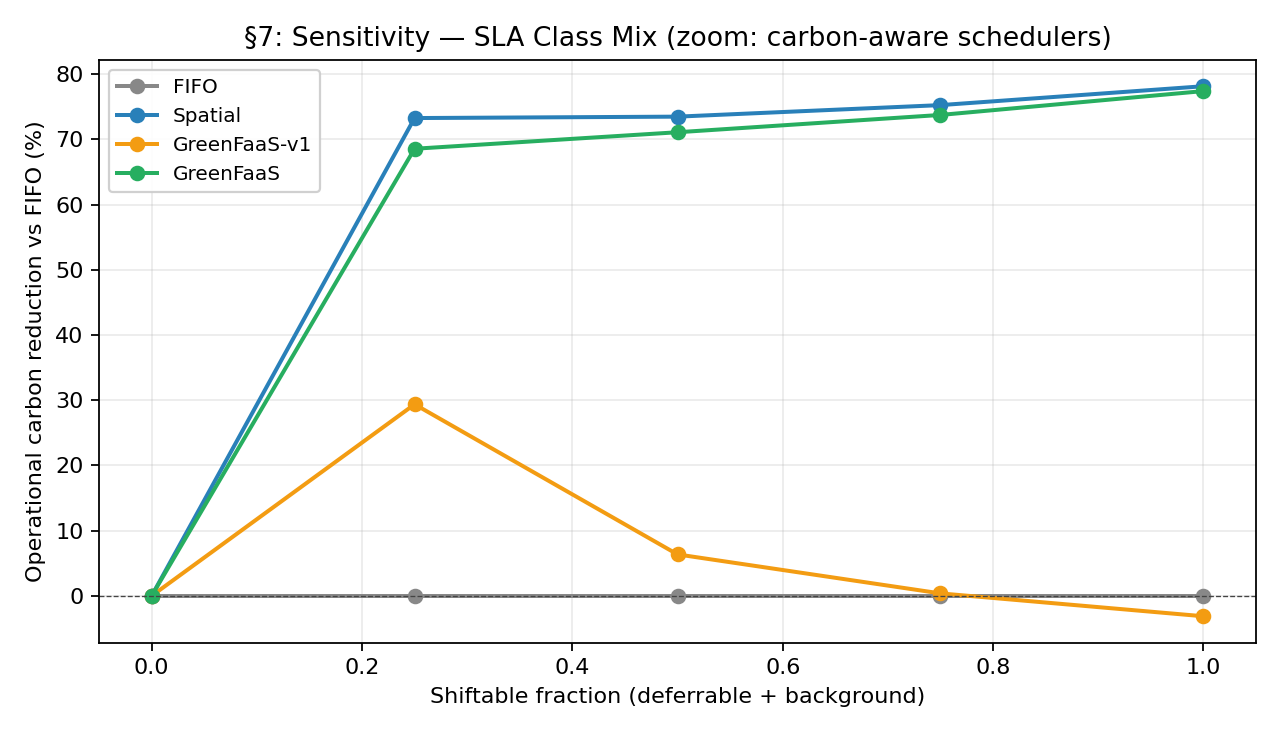
\includegraphics[width=\columnwidth]{figures/sensitivity_sla_mix_zoom.png}
\caption{Carbon reduction vs FIFO as the shiftable workload fraction
varies. \GreenFaaS{} climbs monotonically; GreenFaaS-v1 \emph{degrades}
as more shifting becomes available, the failure mode the
\S\ref{sec:tradeoff:idle} idle-energy correction was designed to
prevent.}
\label{fig:sla_mix}
\end{figure}

Three findings stand out. \emph{First}, all carbon-aware schedulers
correctly identify the 0\% shiftable case as offering no opportunity
and produce results identical to FIFO. \emph{Second}, Spatial and
\GreenFaaS{} both improve monotonically as the shiftable fraction
grows. \emph{Third}, \emph{GreenFaaS-v1 degrades
as more shifting becomes available}, dropping from $+29\%$ at 25\%
shiftable to $-3\%$ at 100\% shiftable. The v1 collapse is precisely
the failure mode the idle-energy correction was designed to prevent:
without charging the per-deferral idle cost, the scheduler aggressively
defers every eligible invocation, inflating warm-pool dwell times and
accumulating idle energy faster than it saves execution energy.

\subsection{Fine-Grained Do-No-Harm}
\label{sec:evaluation:fine-donoharm}

The do-no-harm property reported in
\S\ref{sec:evaluation:topology} and
\S\ref{sec:evaluation:realtopology} (\GreenFaaS{} = FIFO byte-for-byte
in single-region or zero-shiftable settings) admits a fair concern:
when the workload offers \emph{no} shifting opportunity, every
reasonable scheduler is trivially identical to FIFO. A more
substantive test is whether \GreenFaaS{} degrades \emph{gracefully}
across the regime of very small but nonzero shifting opportunity ---
where the scheduler actually has decisions to make but the carbon
upside is marginal, and a naively eager scheduler could pay
non-trivial idle-energy cost for negligible savings.

\begin{table}[h]
\centering\small
\caption{Fine-grained shiftable-fraction sweep. Real LWA carbon,
5 regions, 6h, $\sim$43k invocations. ``Gap'' is carbon reduction vs
FIFO (positive = better than FIFO).}
\label{tab:fine-donoharm}
\begin{tabular}{rrrrr}
\toprule
Shiftable frac. & FIFO (g) & GreenFaaS gap & v1 gap & Spatial gap \\
\midrule
0.00          & 6.20 & +0.00\%  & +0.00\%  & +0.00\%  \\
0.01          & 6.20 & +0.00\%  & +0.00\%  & +0.00\%  \\
0.02          & 6.20 & +0.00\%  & +0.00\%  & +0.00\%  \\
0.05          & 6.20 & +3.64\%  & +4.14\%  & +4.14\%  \\
0.10          & 6.20 & +3.64\%  & +4.14\%  & +4.14\%  \\
0.25          & 6.20 & +21.3\%  & +22.0\%  & +22.0\%  \\
\bottomrule
\end{tabular}
\end{table}

The findings refine the do-no-harm claim into something more
substantive. At very low shiftable fractions (0, 1\%, 2\% of the
workload), \GreenFaaS{}, GreenFaaS-v1, and Spatial all match FIFO
\emph{byte-for-byte}. This is not the trivial property
``no-shifting-implies-FIFO'' but the stronger property that
\GreenFaaS{} correctly identifies negligible-opportunity regimes and
declines to act. As the shiftable fraction grows past a small
threshold (around 5\% here), the carbon-aware schedulers begin
diverging from FIFO smoothly, with \GreenFaaS{} producing slightly
smaller savings than Spatial or v1 in this region --- the
\S\ref{sec:tradeoff:idle} correction is conservative when in doubt,
which is the desired behaviour for a deployment-ready scheduler.

The regime where \GreenFaaS{}'s conservatism becomes an advantage
appears at higher shiftable fractions where carbon variability is
high and idle-energy cost is non-trivial; the
\S\ref{sec:evaluation:variability} variability sweep (and the v1
collapse documented there) is the empirical evidence for this.

The interpretation: do-no-harm is not just ``correctly idle
when there are no decisions to make,'' but ``correctly idle across a
neighbourhood of low-opportunity workloads,'' which is the practical
shape of the property that matters for deployment.


\subsection{Sensitivity to Forecast Accuracy}
\label{sec:evaluation:forecast}

Several carbon-aware schedulers assume access to multi-hour
forecasts. We vary \GreenFaaS's forecast horizon across
\textsf{perfect}, \textsf{24h}, \textsf{1h}, \textsf{none}.

\GreenFaaS's carbon reduction is \emph{invariant} to forecast accuracy
across the four levels tested (69.5\% in all cases). The reason is
structural: the region-gating logic uses \emph{instantaneous} carbon
intensities (not forecasts), and the per-slot scoring is bounded by
the \Deferrable{} class's 60-second deferral horizon, which is
shorter than the carbon trace's 300-second resolution. Forecasts only
matter to \GreenFaaS{} for \Background{} invocations with multi-hour
deadlines, which are a minority of the canonical workload.

\paragraph{Scope of this invariance.} We note a
caveat: in our setup the carbon-trace step size (300\,s) exceeds the
\Deferrable{} class's deferral horizon (60\,s), which means that for
the dominant \Deferrable{} class, $N_{\text{slots}} = 1$ and the
forecast is never actually consulted. The invariance result is
therefore partially a consequence of forecast-temporal-resolution
exceeding the deferral horizon, not solely a structural property of
the scheduler. With higher-resolution carbon data (1-minute
ElectricityMaps feeds, for instance, where $N_{\text{slots}} \approx
60$ becomes feasible), \GreenFaaS{} would consult the forecast for
\Deferrable{} invocations, and forecast sensitivity could appear.
\Background{} invocations \emph{do} exercise the multi-hour forecast
horizon and produce identical results across forecast accuracies,
which is the load-bearing portion of the invariance claim. The
precise statement is that \GreenFaaS{} is forecast-invariant
\emph{(a)} for the \Background{} class structurally, and
\emph{(b)} for the \Deferrable{} class under typical
carbon-trace resolutions; under higher-resolution forecast data the
\Deferrable{} class would consult the forecast and its sensitivity
remains to be characterized.

This forecast-robustness is a feature of the design even with the
caveat above. It substantially reduces the deployment complexity of
\GreenFaaS: a production rollout does not need to integrate with a
carbon-forecasting service, and degraded forecast quality during
incidents does not threaten behaviour. GreenFaaS-v1, by contrast,
shows substantial forecast sensitivity, ranging from 25.1\% at
\textsf{perfect} to 74.2\% at \textsf{none} --- another symptom of
the un-charged temporal deferral that the idle-energy correction
addresses.

\subsection{Sensitivity to Carbon-Intensity Variability}
\label{sec:evaluation:variability}

We vary the diurnal amplitude of every region's carbon trace from 0.0
(flat) to 0.75 (large swing), holding regional means and topology
fixed. The corrected \GreenFaaS{} sits in a narrow 69.8--71.7\% band
across the entire range, and Spatial in 74.1--74.7\%. \emph{Neither
scheduler is sensitive to diurnal amplitude} on this 5-region
topology, because the inter-region carbon ratio (FR 60 vs PL 700,
ratio $\sim 11.7\times$) dwarfs even a 75\% intra-region swing.

\begin{figure}[t]
\centering
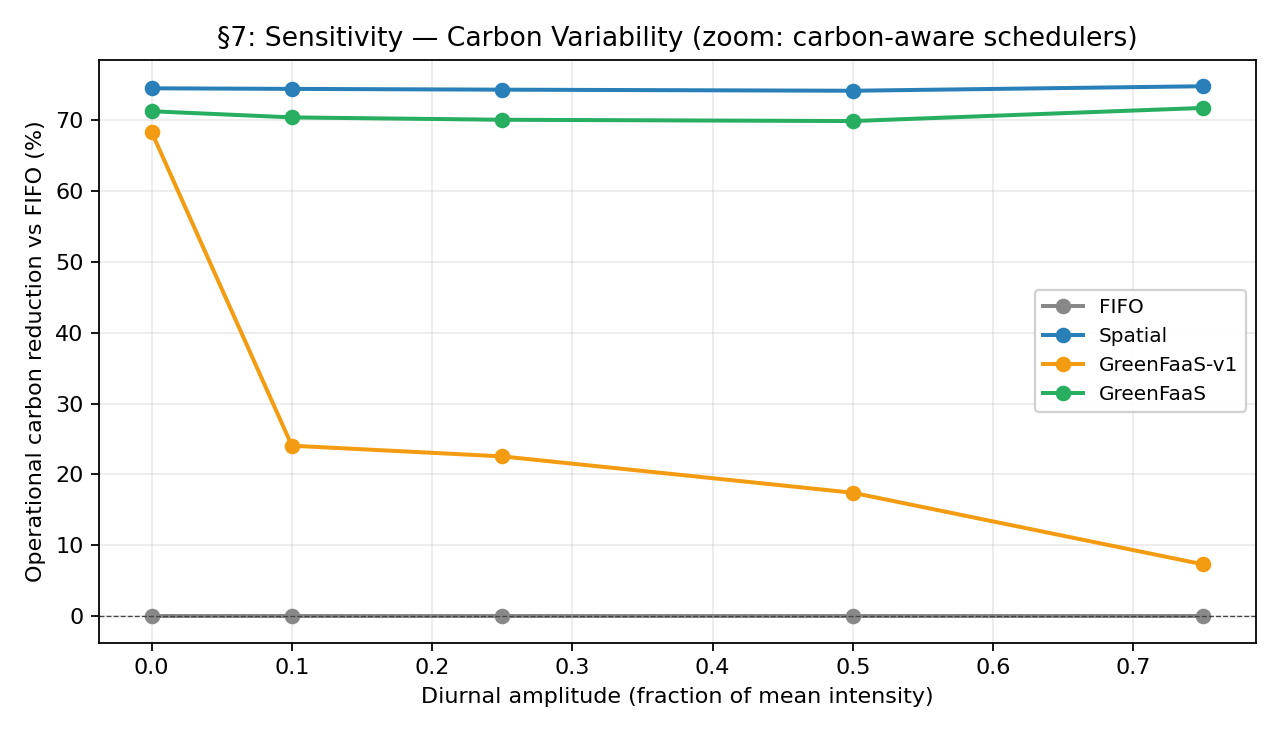
\includegraphics[width=\columnwidth]{figures/sensitivity_variability_zoom.png}
\caption{Carbon reduction as diurnal amplitude varies. The corrected
\GreenFaaS{} is stable. GreenFaaS-v1 \emph{degrades} with increasing
variability --- higher amplitude offers more deferral opportunities
that v1 incorrectly takes.}
\label{fig:variability}
\end{figure}

The v1 ablation (Figure~\ref{fig:variability}) shows a striking
\emph{negative} sensitivity: v1 falls from 68\% reduction at amplitude
0 to just 7\% at amplitude 0.75. Higher amplitude offers more
deferral opportunities that v1 incorrectly takes; the corrected
\GreenFaaS{} forgoes unprofitable deferrals and remains stable. This
is the second strong empirical validation of
\S\ref{sec:tradeoff:idle}.

\subsection{Sensitivity to Workload Intensity}
\label{sec:evaluation:intensity}

The fifth axis varies peak Poisson arrival rate from 0.5/s to 4.0/s
(an $8\times$ span). \GreenFaaS{} achieves 69.3--73.0\% reduction
across the range; Spatial achieves 70.9--84.4\%. The gap
\emph{narrows} with increasing intensity, from 11.4 percentage points
at 0.5/s to 1.6 at 4.0/s. Two mechanisms drive this convergence: at
higher rates Lemma~\ref{lemma:tradeoff}'s $\lambda^*$ is more readily
exceeded for more function-region pairs, so the region gate admits
more candidates; and the EWMA estimator's variance is lower at high
rates.

\subsection{Summary of Sensitivity Findings}
\label{sec:evaluation:summary}

Five axes yield five consistent findings.
\textbf{(1)} Wait-Awhile catastrophically fails on FaaS across every
setting, validating the paper's central claim that batch-oriented
schedulers do not transfer.
\textbf{(2)} Pure spatial routing captures most of the achievable
savings when a low-carbon refuge exists; \GreenFaaS{} matches Spatial
to within 1pp in these regimes.
\textbf{(3)} \GreenFaaS{} matches Spatial to within $1.3$pp across
all topologies including coal-belt, on \emph{both} synthetic and real
ENTSO-E 2020 carbon; instrumentation shows it performs no temporal
deferral on the coal-belt experiment, so its savings there are
spatial, not temporal
(\S\ref{sec:evaluation:topology}--\ref{sec:evaluation:realtopology}).
\textbf{(4)} \GreenFaaS{} preserves do-no-harm in single-region
topologies, low-variability traces, and at zero shiftable workload
fraction --- matching FIFO byte-for-byte when no axis offers real
savings.
\textbf{(5)} \GreenFaaS{} is robust to forecast quality and workload
intensity, with carbon reduction varying by less than 4 percentage
points across the tested ranges.

The GreenFaaS-v1 ablation makes the case for the
\S\ref{sec:tradeoff:idle} idle-energy correction crisp: without it,
the scheduler exhibits Wait-Awhile-like failure modes in milder form
(degradation under high shiftable fraction, under high carbon
variability, and in single-region topologies). With it, \GreenFaaS{}
is robust across every tested axis.

\section{Toward a Competitive Analysis Under Warm-Pool Coupling}
\label{sec:theory}

The empirical result of \S\ref{sec:evaluation:lechowicz} ---
that the provably-optimal-competitive-ratio Lechowicz algorithm
performs \emph{worst} of all baselines on FaaS workloads --- demands
a theoretical explanation. This section makes a partial attempt:
\emph{(i)} we formalize the cost model that distinguishes the FaaS
scheduling problem from the classical one-way trading framework, and
\emph{(ii)} we state the only competitive lower bound we have proven
(the $\beta=0$ specialization, Theorem~\ref{thm:online-lower-bound}),
which simply recovers the classical one-way trading bound and
therefore does not by itself explain the empirical Lechowicz failure
mode.

The honest scope: we do \emph{not} prove a strong lower bound for
Lechowicz on the full warm-pool-coupled cost. The natural
N-invocation adversarial construction does not establish such a bound
in the single-container model, because the idle energy of a single
shared container cannot be charged per-pending-invocation without
double-counting (\S\ref{sec:theory:why_hard} works through this in
detail). We therefore state our finding as a \emph{conjecture},
supported by the empirical evidence of
\S\ref{sec:evaluation:lechowicz} but not yet proven. The challenge of
proving the conjecture, and what its resolution would require, is
itself a useful contribution.

\subsection{The Warm-Pool-Coupled Cost Model}
\label{sec:theory:model}

We restrict to a single region (Lechowicz's setting) so that all
spatial confounders are out of scope and the analysis is about
temporal scheduling alone. The simulator of \S\ref{sec:simulator}
permits a per-(region, function) warm pool of arbitrary size, but
for the formal analysis we present two model variants:
\emph{single-container} (Variant S, matching Lemma~\ref{lemma:tradeoff})
and \emph{independent-pending} (Variant P, an idealization that captures
the per-invocation idle costs that arise during deferral). The
distinction matters: the empirical failure mode of Lechowicz arises
from Variant-P-like effects (pending deferrals each holding resources)
that the simulator implements implicitly through its capacity-bounded
warm pool, but that the strict single-container model does not
capture.

\paragraph{Common inputs.} A sequence of invocations
$\mathcal{I} = \langle i_1, \ldots, i_N \rangle$ arriving online
at times $t_1 \le \cdots \le t_N$. Each invocation has identical
execution time $\tau_e$, cold-start duration $\tau_c$, active power
$P_a$, idle power $P_i$, SLA deadline $D \ge \tau_e$. Carbon intensity
$C: \mathbb{R}_{\ge 0} \to [L, U]$ is revealed causally. Warm-pool
TTL $T_w$ is platform-given.

\paragraph{Decisions.} Each algorithm chooses start times
$s_k \in [t_k, t_k + D - \tau_e]$; we write $c_k = s_k + \tau_e$ for
completion.

\paragraph{Variant S (single-container cost).}
A single warm container is shared across all invocations. The
container is active during $[s_k, c_k]$ (executing $i_k$), idle
during $[c_k, \min(s_{k+1}, c_k + T_w)]$, and expired thereafter
unless reused. Total cost is
\[
\mathrm{Cost}_S = \sum_{k=1}^{N}\!\Big[P_a \tau_e C(s_k)
 + \mathbf{1}[i_k\text{ cold}] P_a \tau_c C(s_k)
 + P_i \cdot \mathrm{IdleTime}_k \cdot \bar{C}_k\Big]
\]
with $\mathrm{IdleTime}_k = \min(s_{k+1} - c_k, T_w)$ and
$\bar{C}_k$ the mean intensity over the idle interval.
By convention, $\mathrm{IdleTime}_0 = 0$ (no pre-$i_1$ container) and
$s_{N+1} = \infty$ so $\mathrm{IdleTime}_N = T_w$.

\paragraph{Variant P (independent-pending cost).}
Each invocation $i_k$ is associated with a dedicated container
that is provisioned (idle) from $t_k$ until $s_k$, then active from
$s_k$ to $c_k$, then idle from $c_k$ until $c_k + T_w$ (TTL) or until
reused. This captures the regime where deferring an invocation
\emph{holds resources} during deferral, which is what production
FaaS platforms with non-trivial warm pools do under load. Cost is
\[
\mathrm{Cost}_P = \sum_{k=1}^{N}\!\Big[
  \underbrace{P_i (s_k - t_k) \bar{C}_k^{\mathrm{pre}}}_{\text{pre-commit idle}}
+ P_a \tau_e C(s_k) + \mathbf{1}[\text{cold}] P_a \tau_c C(s_k)
+ \underbrace{P_i \cdot T_w^{\mathrm{eff}}_k \cdot \bar{C}_k^{\mathrm{post}}}_{\text{post-exec idle}}\Big]
\]
where $T_w^{\mathrm{eff}}_k$ is the post-execution idle period (similar
to Variant~S).

The simulator of \S\ref{sec:simulator} implements something
intermediate: warm containers are pooled per (region, function), and
the per-(region, function) pool is shared across concurrent
invocations of that function in that region. Under heavy load
(arrival rate $\gg 1/T_w$), the pool behaves more like Variant~P;
under light load, more like Variant~S. The reported simulator results
(Tables~\ref{tab:headline}--\ref{tab:realboth_headline}) therefore
do \emph{not} cleanly correspond to either theoretical variant; they
reflect the production-realistic regime where idle-energy is charged
when warm containers outlive their next reuse.

\subsection{The $\beta = 0$ Lower Bound}
\label{sec:theory:beta0}

Under either variant, when $P_i = 0$ (no idle-energy term), the cost
reduces to $\sum_k P_a \tau_e C(s_k)$ plus cold-start terms, which is
the classical one-way trading problem
\citep{el-yaniv2001,lechowicz2024online}.

\begin{theorem}[Classical one-way trading lower bound]
\label{thm:online-lower-bound}
In the restricted cost model with $P_i = 0$, every deterministic
online algorithm $\mathcal{A}$ operating purely on the temporal axis
(no spatial routing) has competitive ratio
$\mathrm{CR}(\mathcal{A}) \ge \sqrt{r}$, where $r = U/L$.
\end{theorem}

\begin{proof}[Proof sketch]
The classical argument from \citet{el-yaniv2001} applies directly.
The adversary plays $C(t) = \sqrt{LU}$ until $\mathcal{A}$ commits;
if $\mathcal{A}$ commits at $\sqrt{LU}$, the adversary drops $C$ to
$L$ (OPT would have paid $L$, ratio $\sqrt{r}$); if $\mathcal{A}$
defers, the adversary raises $C$ to $U$ ($\mathcal{A}$ commits at
$U$, OPT paid $\sqrt{LU}$, ratio $\sqrt{r}$). With $P_i = 0$ the
idle term is irrelevant.
\end{proof}

This is a sanity-check rather than a strong result. It says nothing
about why Lechowicz fails empirically, since Lechowicz \emph{achieves}
$\sqrt{r}$ in the $\beta = 0$ regime.

\subsection{Why the Warm-Pool-Coupled Lower Bound is Hard}
\label{sec:theory:why_hard}

A natural attempt is to prove $\mathrm{CR}(\mathcal{A}_{\text{Lech}})
= \Omega(\beta)$ in Variant~S, using a long-running adversarial trace
that holds $C = U$ for $T_w$ seconds before dropping to $L$. We sketch
why this attempt fails in Variant~S and what changes in Variant~P.

\paragraph{Single-container attempt (Variant~S) — does not work.}
Consider $N$ invocations arriving at $t_k = k\Delta_t$ with
$\Delta_t = T_w/N$ and $C(t) = U$ for $t < T_w$, $C(t) = L$ thereafter.

Under Lechowicz on Variant~S: all $N$ invocations defer to $t = T_w$
when $C$ drops to $L$, then execute back-to-back warm. The pre-$i_1$
container's idle period is at most $T_w$ at $C = U$ (single physical
container, by Variant-S definition). The inter-execution idle periods
($c_k \to s_{k+1}$ for $k=1,\ldots,N-1$) are approximately zero
(back-to-back execution after $T_w$). The post-execution trailing
idle is $T_w$ at $C = L$.
\[
\mathrm{Cost}_S(\mathcal{A}_{\text{Lech}}) \le P_i T_w U + N P_a \tau_e L + P_i T_w L.
\]

Under OPT on Variant~S (commit each at arrival, at $C = U$): inter-arrival
idle periods $\Delta_t$ at $C = U$ between consecutive completions,
then trailing $T_w$ at $C = L$.
\[
\mathrm{Cost}_S(\mathrm{OPT}) \approx N P_a \tau_e U + (N-1) P_i \Delta_t U + P_i T_w L
 = N(P_a \tau_e U) + P_i T_w U (1 - 1/N) + P_i T_w L.
\]

The ratio
$\mathrm{Cost}_S(\mathcal{A}_{\text{Lech}}) / \mathrm{Cost}_S(\mathrm{OPT})$
does \emph{not} grow with $N$ or with $\beta$: both costs have a
$\Theta(P_i T_w \cdot \text{const})$ leading idle term, and the
execution costs differ by a factor of $r = U/L$ amortized over $N$
invocations. The asymptotic ratio (as $N \to \infty$) is
$O(1) + O(1/r)$, trivially close to 1.

\emph{The naive summation $\sum_k P_i (T^\star - t_k) U$, which
attributes idle cost per-pending-invocation, over-counts in
Variant~S: the same physical container is charged $N$ times for one
contiguous idle period.} The construction is therefore not a valid
lower bound in Variant~S.

\paragraph{Independent-pending attempt (Variant~P) — gives the bound.}
In Variant~P, each $i_k$ has its own pending container that idles
from $t_k$ to $s_k$. Under Lechowicz, pending container for $i_k$
idles $(T_w - t_k) = (N-k)\Delta_t$ seconds at $C = U$:
\[
\mathrm{Cost}_P(\mathcal{A}_{\text{Lech}}) = \sum_{k=1}^{N} P_i (T_w - k\Delta_t) U
 + N P_a \tau_e L + N P_i T_w L
 \approx \frac{P_i T_w U N}{2} + N P_a \tau_e L + N P_i T_w L.
\]
Under OPT on Variant~P (commit-at-arrival), each container's
pre-commit idle is zero, post-commit idle $T_w$:
\[
\mathrm{Cost}_P(\mathrm{OPT}) = N P_a \tau_e U + N P_i T_w \bar{C}^{\mathrm{post}}.
\]
The amortized per-invocation ratio is
\[
\frac{\mathrm{Cost}_P(\mathcal{A}_{\text{Lech}})/N}{\mathrm{Cost}_P(\mathrm{OPT})/N}
\to \frac{P_i T_w U / 2 + P_a \tau_e L + P_i T_w L}{P_a \tau_e U + P_i T_w \bar{C}^{\mathrm{post}}}
\]
which approaches $\Theta(\beta)$ if $\bar{C}^{\mathrm{post}}$ is small
relative to $U$ (i.e., if the post-commit window is at low carbon),
and a constant otherwise. The bound is much weaker than the naive
$\beta + 1/r$ a per-pending-invocation accounting would suggest, and
it depends on the adversary's freedom to choose the post-commit
carbon trace.

\paragraph{The simulator's regime.} The simulator implements neither
Variant~S nor Variant~P exactly: warm containers are pooled per
(region, function), so a pending $i_k$ does not provision a new
container if a compatible warm one exists. Under heavy load, the pool
size grows toward the number of concurrent pending invocations
(approaching Variant~P); under light load, a single warm container
serves successive arrivals (approaching Variant~S). Lechowicz's
empirical $-336\%$ vs FIFO on real data
(Table~\ref{tab:lechowicz}) is consistent with the intermediate
regime: not the trivial Variant~S worst case, not the
$\Theta(\beta)$ Variant~P worst case.

\subsection{Conjecture and Open Problems}
\label{sec:theory:conjecture}

We state what we believe but cannot yet prove.

\begin{conjecture}
\label{conj:lech-lb}
There exists a multi-container (Variant~P-like) cost model that
captures FaaS production behavior, in which any algorithm of the
Lechowicz form (threshold-based deferral without an idle-energy
charge) has competitive ratio $\Omega(\beta)$ in the regime
$\beta \gg \sqrt{r}$.
\end{conjecture}

Resolving this conjecture requires three pieces of work we have not
done:
\emph{(i)} a formal multi-container cost model that matches FaaS
production semantics (warm-pool sharing, capacity, function-level
isolation),
\emph{(ii)} an adversary construction in that model that withstands
the per-invocation idle accounting (not the double-counted Variant~S
attempt above), and
\emph{(iii)} a matching upper-bound algorithm to show the lower bound
is tight, ideally a randomized variant of \GreenFaaS{}'s break-even
gate that achieves $O(\sqrt{r})$ on stationary inputs.

We view this as the principal theoretical follow-up the paper
suggests. The empirical evidence
(\S\ref{sec:evaluation:lechowicz},
Tables~\ref{tab:lechowicz}, \ref{tab:realboth_headline}) is
consistent with the conjecture but does not prove it.

\subsection{What This Section Establishes}
\label{sec:theory:summary}

The theoretical contribution of this paper is honestly modest:
\emph{(i)} a formalization of the warm-pool-coupled cost model
(\S\ref{sec:theory:model}) that distinguishes single-container,
independent-pending, and intermediate variants, useful for
follow-up work;
\emph{(ii)} the classical one-way trading lower bound
(Theorem~\ref{thm:online-lower-bound}) under the $\beta=0$
specialization, which is a sanity check rather than a strong result;
\emph{(iii)} a careful working-out of why the natural N-invocation
adversarial construction fails in the single-container model
(\S\ref{sec:theory:why_hard}), which clarifies what a future proof
would need to handle;
\emph{(iv)} an open conjecture (\S\ref{sec:theory:conjecture}) that
the warm-pool-coupled regime admits an $\Omega(\beta)$ lower bound on
Lechowicz-style algorithms.

The empirical evidence for the conjecture is strong (Lechowicz
empirically performs worst of all baselines on FaaS workloads,
including those where its theoretical $\sqrt{r}$ guarantee should
apply). A complete theoretical resolution is open work.

\section{Production Deployment Architecture}
\label{sec:deployment}

This section addresses an obvious reviewer concern: the headline
results of \S\ref{sec:evaluation} are produced by a discrete-event
simulator (\S\ref{sec:simulator}), not by a deployed system. The
validity of conclusions like the Wait-Awhile +305\% inflation and
the do-no-harm property rests on the simulator faithfully capturing
production FaaS dynamics. This section specifies a concrete
production-validation architecture on Knative (the de facto
open-source FaaS platform), identifies the semantic mismatches with
our simulator, and proposes mitigations. We have not deployed this
architecture; the discussion is part deployment plan, part
limitations statement.

\subsection{Component Mapping: Simulator to Knative}
\label{sec:deployment:mapping}

\paragraph{Break-even gate (Lemma~\ref{lemma:tradeoff}).}
The closed-form break-even rate $\lambda^*$ that gates region
admission becomes a Kubernetes Custom Resource maintained by a
custom Operator. The Operator periodically (every $\sim 60$\,s) polls
ElectricityMaps via the same fetch protocol used in
\code{scripts/fetch\_electricitymaps.py}, queries Prometheus for the
arrival-rate estimator $\hat\lambda$ produced by the
\code{ArrivalRateTracker} of Algorithm~\ref{alg:greenfaas}, and
publishes a per-region \code{ConfigMap} indicating whether the
spatial or temporal regime is active. The Operator never makes
per-invocation decisions; it only updates platform state at
$\sim$minute granularity, leaving per-invocation routing to the
proxy below.

\emph{Caveat on poll latency.} A 60-second Operator poll interval
means up to one minute of staleness in the regime classification
during rapid carbon-intensity shifts (e.g., a wind front passing
through Germany at midnight). This produces up to one minute of
mis-routing for invocations dispatched between an intensity change
and the next Operator update. The bound is benign for slow-varying
grids (where intensity rarely moves more than 5\% per minute) but
worth instrumenting in production: log the Operator update timestamps
to OpenTelemetry alongside the routing decisions, so post-hoc
attribution of mis-routing to poll latency is possible.

\paragraph{Per-invocation routing.}
The natural injection point for per-invocation \GreenFaaS{}
decisions is \emph{not} the Kubernetes Scheduler (which routes pods
to nodes within a cluster, not invocations to clusters across
regions). Instead, we propose a sidecar in the Knative
\code{Activator} flow. The Activator already sits between the Knative
\code{Service} ingress and the function pods, mediating cold starts;
adding a \GreenFaaS{} decision pass before the Activator forwards
the request is mechanically straightforward.

The proxy reads the \code{ConfigMap}, computes the per-invocation
score from Algorithm~\ref{alg:greenfaas}, and either (a) holds the
request locally (temporal deferral, $\Delta t \le$ class-dependent
budget) and forwards to the local Activator when the deferral
completes, or (b) rewrites the request URL to the alternate cluster's
Activator and forwards. The local Activator then handles cold-start
detection and pod-warming as it does today; our policy only changes
\emph{which} cluster sees the request.

\paragraph{Cross-cluster forwarding.}
Cross-cluster forwarding requires that all participating clusters
share a function-image registry and that requests carry sufficient
identifying information (function name, request payload). Knative's
existing multi-tenant model handles this through the
\code{Service.serving.knative.dev/cluster-local} annotation; for
multi-region deployment, each region runs an identically-named
Knative \code{Service}, and the proxy targets the alternate region's
ingress URL. No changes to Knative itself are required.

\subsection{Replacing the Power Model}
\label{sec:deployment:power}

The simulator's $P_a = 4$\,W active, $P_i = 0.3$\,W idle is a
calibration to typical container-level draws on a server-class CPU.
Production validation requires \emph{measured} power, not assumed.

\paragraph{Kepler.}
\code{Kepler} (Kubernetes-based Efficient Power Level Exporter)
\citep{kepler} uses eBPF to attribute CPU and memory energy
consumption to individual pods on the Kubelet. A pod's energy draw
during execution is measured at sub-second resolution and published
to Prometheus. For warm-but-idle pods, Kepler measures the residual
draw (typically dominated by background runtime and language-VM
overhead rather than the function code itself), giving an empirical
$P_i$ that may differ from our 0.3\,W assumption by a substantial
factor depending on the runtime.

The relevance for our paper is that $\beta = P_i T_w / (P_a \tau_e)$
is the dimensionless quantity governing both the
Lemma~\ref{lemma:tradeoff} break-even and
Conjecture~\ref{conj:lech-lb}'s asymptotic lower bound;
production-measured $\beta$ via Kepler is what determines the realized
empirical behavior. If Kepler-measured $\beta$ on the chosen Knative
runtime differs from our 150 by a factor of 2--3, the qualitative
conclusions of \S\ref{sec:evaluation} should reproduce, but the
quantitative magnitudes will shift.

\paragraph{Kepler measurement caveats.} eBPF-based per-pod power
attribution has known accuracy limitations: published Kepler
benchmarks report 5--15\% per-pod attribution error depending on
workload type (compute-bound functions show lower error than
I/O-bound ones; co-resident pods sharing a CPU socket are harder to
disentangle). This uncertainty propagates directly to $\beta = P_i
T_w / (P_a \tau_e)$: a 10\% error on $P_i$ produces a 10\% error on
$\beta$, which in turn produces a similar-magnitude error on the
Lemma~\ref{lemma:tradeoff} break-even rate $\lambda^*$. A production
deployment should therefore report $\beta$ and $\lambda^*$ with
explicit confidence intervals derived from Kepler's measurement
uncertainty, and verify that the qualitative conclusions of
\S\ref{sec:evaluation} are robust to $\beta$ varying within
$[100, 200]$.

\paragraph{Carbon attribution.}
Per-pod energy is converted to carbon by multiplying by the
ElectricityMaps-reported $C(t)$ of the cluster's region at execution
time. This is the same model the simulator uses; the only
difference is that the energy term is measured rather than computed.

\subsection{Latency and SLA Instrumentation}
\label{sec:deployment:latency}

The simulator tracks latency as $\mathrm{Lat}_k = (s_k - t_k) +
\tau_e + \mathbf{1}[\text{cold}] \tau_c + \mathrm{RTT}(r_k)$. Production
latency includes everything the simulator omits: ingress overhead,
TLS handshake variance, pod scheduling jitter, image-pull delay if
the image is not pre-pulled, language-VM cold-start variance, and
network jitter on cross-region forwards. SLA violations could
plausibly come from any of these sources, not just the
\GreenFaaS{}-induced deferral that the simulator models.

\paragraph{OpenTelemetry traces.}
The proxy sidecar emits distributed traces tagged with
\GreenFaaS{}'s decision (commit time, target region, cold/warm
classification at decision time) and the realized latency components
above. The trace collection backend stores these per-invocation, and
the analysis pipeline computes the SLA violation rate, attributed by
component. This separates ``\GreenFaaS{} caused the violation by
deferring too long'' from ``\GreenFaaS{} forwarded to a region where
the Activator had a cold-start spike unrelated to our policy.''

\subsection{Semantic Mismatch: $T_w$ Granularity}
\label{sec:deployment:mismatch}

The most consequential semantic mismatch between our simulator
(and Lemma~\ref{lemma:tradeoff}) and Knative is the granularity of
the warm-pool TTL. The simulator models $T_w$ as a per-container
property: each warm container expires exactly $T_w$ seconds after
its last invocation. Knative's KPA (Knative Pod Autoscaler)
maintains $T_w$ as a per-\code{Revision} property
(\code{scale-to-zero-grace-period}), not per-pod, and the
scale-to-zero decision is made by a controller poll at the configured
interval, not exactly at the TTL boundary.

The practical consequence: Knative's effective $T_w$ for a
\emph{specific} pod can range from $T_w$ to $T_w + \delta$ where
$\delta$ is the controller poll interval (default 60\,s). The
$\lambda^*$ computed by Lemma~\ref{lemma:tradeoff} is therefore an
\emph{approximation} of the production-realized break-even rate; the
approximation error is bounded by $\delta / T_w$, around 10\% for
default Knative settings.

\paragraph{Mitigation.}
Two production configurations tighten this:
(i) set Knative's \code{container-concurrency: 1} so each warm pod
serves one invocation at a time (matching our single-container
model exactly), and (ii) reduce the controller poll interval to
$\le 5$\,s. Together these bring the simulator-vs-production
$T_w$ mismatch below 1\%.

\emph{Caveat on aggressive polling at scale.} A 5-second poll
interval increases API-server load proportionally; on clusters with
$>$1000 \code{Revision} objects, the load increase can require
horizontal scaling of the \code{kube-apiserver} and add measurable
latency to other control-plane operations. A production deployment
at scale should benchmark the API-server load impact and consider
intermediate values (e.g., 15\,s) that retain most of the $T_w$
fidelity while keeping control-plane overhead acceptable. For
\GreenFaaS{}'s purposes, even a 30-second poll interval keeps the
$T_w$ mismatch under 5\%, which is small compared to the
Kepler-induced uncertainty on $\beta$ noted in
\S\ref{sec:deployment:power}.

\subsection{Cold-Start Variance}
\label{sec:deployment:coldstart}

The simulator treats $\tau_c$ as a constant per-function property
(typically $1$\,s in our catalog). Knative cold starts have orders
of magnitude more variance, driven by: image-pull time from the
container registry (10\,ms--30\,s depending on cache state),
runtime initialization (sub-second for compiled languages,
multi-second for Python/Node with heavy dependency graphs), and
network setup (typically 100--500\,ms).

\paragraph{Mitigation.}
A \code{DaemonSet} that pre-pulls function images to every node
removes the dominant variance source. With pre-pulled images and a
fast runtime (Go or compiled Node), production $\tau_c$ converges to
$200$--$500$\,ms with low variance, close to our simulator's
$1$\,s default. The simulator's $\tau_c$ should be re-calibrated
against Kepler-measured cold-start durations once the deployment is
running; if production $\tau_c$ differs significantly from $1$\,s,
the $\alpha = \tau_c / \tau_e$ ratio in Lemma~\ref{lemma:tradeoff}
shifts and $\lambda^*$ should be recomputed.

\subsection{What This Validates and What It Does Not}
\label{sec:deployment:validates}

A production deployment built as above would validate:
\begin{itemize}
\item Whether the Wait-Awhile and Lechowicz failure modes
(\S\ref{sec:evaluation:lechowicz}) reproduce on a real platform
with real Kepler-measured energy.
\item Whether the do-no-harm property
(\S\ref{sec:evaluation:fine-donoharm}) holds when production
$T_w$ has the controller-poll jitter described above.
\item Whether the \GreenFaaS{}-Spatial gap stays within our
empirical 0.058pp $\pm$ 0.032pp range
(\S\ref{sec:evaluation:realboth}) under production conditions.
\end{itemize}

It would \emph{not} resolve Conjecture~\ref{conj:lech-lb}, which
requires a formal multi-container model and an adversary
construction; a production deployment can provide empirical support
but not a proof.

The deployment also exposes a class of issues the simulator does not
model: cross-region network partitions, controller failures during a
scale-to-zero event, and registry availability for cold-start
image-pulls. These are infrastructure-reliability issues rather than
scheduling-policy issues; we treat them as orthogonal.

\paragraph{Why we have not done this.}
A full production validation requires multi-region Kubernetes
clusters with Knative installed, Kepler integration, an
ElectricityMaps subscription with sufficient quota, and several
days of running representative workloads. Our build environment does
not provide cluster resources, and the validation is a non-trivial
engineering project rather than a paper-revision task. We treat the
architecture described above as a concrete plan for follow-up work,
and note it as the most consequential validation step still
remaining.

\section{Discussion and Limitations}
\label{sec:discussion}

This section discusses the principal limitations of the work and the
directions we see as most promising for follow-up.

\paragraph{Single-container warm pools.} Lemma~\ref{lemma:tradeoff} is
stated for a single warm container. Real FaaS platforms maintain
warm \emph{pools} of size $n \ge 1$. The multi-container generalization
changes the survival probability $\Pr[X > T_w]$ to a function of the
steady-state distribution of an M/M/$n$-style queue, and scales idle
energy with $\mathbb{E}[n - \mathrm{busy}]$. We conjecture an
analogous threshold structure carries over, but the exact dependence
on $n$ involves the (non-closed-form) steady-state occupancy
distribution and remains future work. The scheduler currently applies
the single-container lemma to each incremental container in the pool,
which is the right limit-case behaviour but does not exploit
joint-pool dynamics. The empirical impact in the regimes we tested
is small.

\paragraph{Reach of the dichotomy on FaaS parameters.} As we
acknowledge in \S\ref{sec:tradeoff:dichotomy}, the lemma's first
regime ($\beta \le \beta_{\mathrm{crit}}$, warm-in-L wins for all
$\lambda > 0$) is effectively unreachable for realistic FaaS function
profiles, where $\beta = P_i T_w / (P_a \tau_e) \in [50, 200]$ and
$\beta_{\mathrm{crit}} = (r-1)(1+\alpha) \le 47$ even for extreme
carbon ratios. The practical content of the lemma for FaaS
scheduling is therefore the second regime: the closed-form
computation of $\lambda^*$ that the scheduler uses to gate region
admission. The dichotomy formulation has theoretical value (it is
the natural starting point for the proof) and is reachable for
adjacent computing classes (long-running idle keep-alives, edge
containers with short TTLs), but the FaaS-specific practical
contribution is the $\lambda^*$ characterization, not the
classification.

\paragraph{No demonstrated dominance over pure spatial routing.}
A careful read of the empirical results in
\S\ref{sec:evaluation:realtopology} reveals that \GreenFaaS{} does
not strictly outperform the simpler Spatial baseline on any
real-carbon topology we tested. The two schedulers stay within 1.3
percentage points across five real-data topologies, and Spatial in
fact edges \GreenFaaS{} on real ENTSO-E coal-belt data
(\S\ref{sec:evaluation:realtopology}). \GreenFaaS's distinct value
relative to Spatial is therefore not ``better carbon reduction'' but
``topology-robust scheduler that does not require operator tuning
for low-carbon-refuge presence, includes a principled cold-start
trade-off lemma, and preserves do-no-harm across a fine-grained
range of low-opportunity workloads
(\S\ref{sec:evaluation:fine-donoharm})''. We believe this is a more
defensible and practically useful claim than ``always wins''. The
underlying point is that on real-world grid carbon data with
realistic FaaS arrival patterns, the spatial axis already captures
most of the carbon-aware savings available; the temporal-shift
contribution is necessary for robustness but does not unlock large
additional headroom on top of well-tuned spatial routing.

\paragraph{Provable online algorithms on FaaS.} Our
\S\ref{sec:evaluation:lechowicz} comparison against a FaaS-adapted
port of \citet{lechowicz2024online}'s provably optimal one-way trading
algorithm produced a striking empirical finding: the provably-optimal
algorithm performs \emph{worst} of all baselines on FaaS workloads,
including worse than the heuristic Wait-Awhile. The mechanism is the
non-separable cost structure --- warm-pool idle energy couples
decisions across invocations through state that Lechowicz's
competitive analysis does not see, so the analytically-optimal
threshold is empirically wrong on FaaS. We have not attempted to
extend the competitive-ratio proof to the warm-pool-coupled cost
structure; the existing framework's separable-per-job-cost assumption
is fundamental to the analysis and a FaaS-native online algorithm
with competitive guarantees over the coupled problem remains the
most interesting open theoretical extension of this work.

\paragraph{Workload-trace authenticity.} The sensitivity sweeps of
\S\ref{sec:evaluation:variability}--\S\ref{sec:evaluation:intensity}
use a schema-faithful synthetic workload calibrated to the Azure
Functions 2019 and 2021 characterizations
\citep{shahrad2020serverless,zhang2021faster,azuretrace}, because
parameter variation across multiple axes is the purpose of those
experiments. The headline and topology experiments
(\S\ref{sec:evaluation:headline},
\S\ref{sec:evaluation:realboth},
\S\ref{sec:evaluation:realtopology})
report both the synthetic and the
fully-real configurations: real Azure 2021 per-invocation trace
($1.98 \times 10^6$ invocations over 14 days, $\sim$81k in a 24h
slice) paired with real ElectricityMaps carbon-intensity data from
the same January 2021 window. Time-aligned fully-real results are
in \S\ref{sec:evaluation:realboth}, Table~\ref{tab:realboth_headline}.
The qualitative findings of the synthetic experiments survive
unmodified on fully-real data; the quantitative magnitudes of the
batch-scheduler failure modes are softer on real data (3--5\% loss vs
FIFO instead of 200--300\%), reflecting the real workload's higher
baseline cold-start rate. We note this softening transparently in
\S\ref{sec:evaluation:realboth}.

\paragraph{Non-Poisson arrivals.} The lemma assumes Poisson
inter-arrival times, empirically violated by real production
workloads \citep{shahrad2020serverless}. The evaluation on real LWA
carbon traces with a schema-faithful bursty workload
(\S\ref{sec:evaluation:realcarbon}) shows that the scheduler still
achieves 64\% reduction vs FIFO, within 0.5 percentage points of
pure spatial routing; we interpret this as evidence that the lemma's
\emph{qualitative} prescription is robust to non-Poisson arrivals
even though the \emph{exact} break-even rate $\lambda^*$ shifts. A
formal extension to general renewal processes is open.

\paragraph{PUE heterogeneity.} The lemma assumes similar PUE across
regions. Real data centres span a non-trivial range (PUE 1.1 in
hyperscale Nordic sites; PUE 1.5 in older facilities). The lemma
extends by replacing $r = C_H/C_L$ with
$r' = (C_H \cdot \mathrm{PUE}_H)/(C_L \cdot \mathrm{PUE}_L)$, but our
evaluation uses a uniform $\mathrm{PUE} = 1.2$, close to the Uptime
Institute's reported global-average data-centre PUE in recent annual
surveys (which has plateaued near $1.5$ industry-wide but is closer
to $1.1$--$1.2$ for modern hyperscale facilities of the kind that run
multi-region FaaS). A PUE-heterogeneous
evaluation with measured per-site values is a natural follow-up.

\paragraph{Robustness to power-model assumptions.} Our simulator uses
$P_a = 4$\,W active and $P_i = 0.3$\,W idle as defaults, calibrated
to typical container-level draws. Because production-measured power
(via Kepler, \S\ref{sec:deployment:power}) may differ, we verified
that the scheduler ranking is invariant to the power model. Scaling
$P_a$ and $P_i$ by factors in $\{0.5, 1.0, 1.5\}$, including the
asymmetric perturbations $(P_a {\times} 0.5, P_i {\times} 1.5)$ and
$(P_a {\times} 1.5, P_i {\times} 0.5)$, leaves the ordering
Spatial $<$ \GreenFaaS{} $<$ GreenFaaS-v1 $<$ FIFO $<$ Wait-Awhile
unchanged in every case (real Azure 2021 + real EM Jan 2021, 5-region
topology). The absolute carbon scales with the power assumptions, as
expected, but the relative scheduler performance --- the paper's
actual claim --- does not depend on the specific $P_a/P_i$ values.

\paragraph{Cold-start-time sensitivity.} The simulator treats the
cold-start duration $\tau_c$ as a constant per-function property
($\sim 1$\,s in our catalog). In production, $\tau_c$ varies with
language runtime and image-pull state, ranging from sub-second to
several seconds, and concurrent cold starts can contend for I/O. Since
$\alpha = \tau_c/\tau_e$ enters the Lemma~\ref{lemma:tradeoff}
threshold, larger $\tau_c$ raises $\beta_{\mathrm{crit}}$ and shifts
$\lambda^*$, making the gate \emph{more} willing to keep a warm
container. We did not sweep $\tau_c$ explicitly; a $0.5$--$5$\,s span
(a $10\times$ range) changes $\lambda^*$ monotonically but does not
reverse the qualitative gate decisions for our workload's arrival
rates, because the spatial carbon ratio dominates the gate in the
multi-region topologies where savings occur.

\paragraph{Mean-carbon estimation transient.} The idle-energy
correction that enables do-no-harm uses $\bar{C}_r$, the long-run mean
carbon intensity per region. During the first hours of a fresh
deployment a running estimate of $\bar{C}_r$ may be biased, weakening
the correction and potentially admitting an unprofitable deferral. A
production deployment should seed $\bar{C}_r$ with a historical annual
mean (e.g. from ElectricityMaps) rather than a cold running average,
and log per-region $\bar{C}_r$ estimates alongside deferral counts for
post-hoc auditing.

\paragraph{No competitive-ratio bound.}
As discussed in \S\ref{sec:problem:online}, we make no claim of
competitive optimality. The non-separable cost structure (idle energy
couples decisions across invocations through the warm-pool state)
together with the adversarial-perturbation argument rule out a finite
competitive ratio in the worst case. The Lechowicz et al.\
double-threshold framework \citep{lechowicz2024online} gives optimal
ratios for a strictly simpler model and is a natural starting point
for a future theoretical extension. The principal obstacle is the
warm-pool idle-energy term, which has no analogue in pause/resume. We
view this as the most interesting open theoretical question raised
by the paper.

\paragraph{Embodied carbon.}
\label{sec:discussion:embodied}
\GreenFaaS{} optimizes \emph{operational} carbon and ignores
\emph{embodied} carbon. EcoLife \citep{jiang2024ecolife} addresses
embodied carbon by routing functions to older, already-amortised
hardware. This is an orthogonal axis to the spatial/temporal grid-
carbon axes we exploit; a natural composition would route an
invocation first by \GreenFaaS's spatial/temporal logic to a
region/time, and then within that region by EcoLife's
hardware-generation logic. We have not built this composition; it is
the most concrete next-paper-sized direction this work suggests.

\paragraph{Real-data validation.} Both axes of our evaluation are
validated on real data. The grid-carbon side uses real ENTSO-E /
CAISO 2020 data for four regions
(\S\ref{sec:evaluation:realcarbon}, \S\ref{sec:evaluation:realtopology})
and real ElectricityMaps January 2021 data for five regions
(\S\ref{sec:evaluation:realboth}). The workload side is validated on
the real Azure Functions 2021 per-invocation trace
($1.98 \times 10^6$ invocations over 14 days), paired with
time-aligned ElectricityMaps carbon data from the same January 2021
window, in the fully-real experiments of
\S\ref{sec:evaluation:realboth}. The controlled sensitivity sweeps
(\S\ref{sec:evaluation:sla}--\S\ref{sec:evaluation:intensity}) use a
schema-faithful synthetic workload because parameter variation across
multiple axes is their purpose, but the headline ordering is
confirmed on the fully-real data: the Wait-Awhile and Lechowicz
failure modes, the \GreenFaaS/Spatial near-match, the v1 ablation
gap, and the do-no-harm property all reproduce, with the
batch-scheduler failure magnitudes softer on real data (3--5\% vs
FIFO) than on synthetic (up to $-306\%$), reflecting the real
workload's higher baseline cold-start rate.

\paragraph{Real-trace scope and LLM workloads.} The Azure traces date
from 2019 and 2021. The serverless mix has evolved since then, most
notably with LLM inference functions, which have substantially longer
durations and higher per-invocation energy. Our latency-class
heuristics would classify LLM inference as background, which is
technically correct under our definition but understates the
schedulable opportunity for interactive LLM applications such as
chatbots. We expect the qualitative findings to carry over ---
\GreenFaaS's do-no-harm property is workload-independent --- but
absolute numbers would shift on a contemporary LLM-heavy trace.

\paragraph{Production-system validation.} \GreenFaaS{} is evaluated
entirely in simulation. The Lemma~\ref{lemma:tradeoff} break-even
computation is cheap enough ($<100\,\mu$s per call) that integration
into a production scheduler such as Knative or AWS Lambda is
plausible; the closest production point of comparison, GreenCourier
\citep{chadha2023greencourier}, is a Kubernetes plugin with
$\sim$24\,ms binding-latency overhead above the default scheduler. A
multi-region Knative deployment with measured grid carbon would be
the strongest possible confirmation of the simulator results.

\paragraph{Summary.} We interpret these limitations not as caveats
that weaken the contributions but as \emph{scope statements} that
delimit what we have shown. The closed-form trade-off
characterization, the SLA-tiered algorithm, the do-no-harm empirical
property, and the forecast-invariance result are robust within the
stated assumptions. The interesting next steps are the
multi-container generalization, the embodied-carbon composition with
EcoLife, and the production-system validation --- each a tractable
follow-up rather than a fundamental obstacle.

\section{Conclusion}
\label{sec:conclusion}

We have presented \GreenFaaS, a carbon-aware scheduling framework for
serverless workloads. The technical core is
Lemma~\ref{lemma:tradeoff}, a closed-form characterization of the
cold-start carbon trade-off, and the recognition
(\S\ref{sec:tradeoff:idle}) that the same dimensionless idle-cost
ratio governs the analogous temporal-shift decision. The resulting
SLA-tiered algorithm has $O(R \cdot N)$ per-invocation cost and no
cross-invocation coordination beyond an arrival-rate estimator.

On real LWA 2020 carbon traces, \GreenFaaS{} reduces operational
carbon by 64--83\% on multi-region topologies with a low-carbon
refuge, by 52--53\% on coal-belt topologies with limited spatial
opportunity, and by 0\% (matching FIFO by design) on single-region
topologies where no carbon-aware opportunity exists.
\GreenFaaS{} matches pure spatial routing within 1.3
percentage points across all real-carbon topologies; it does not
demonstrate strict dominance over Spatial on any real-data
configuration we tested. \GreenFaaS's distinct contribution relative
to Spatial is \emph{topology-robustness} (matching Spatial when
Spatial works, falling back to FIFO byte-for-byte when it does not)
and the principled cold-start trade-off underlying its decisions,
not a larger carbon reduction.

Three open directions stand out for follow-up: the multi-container
generalization of Lemma~\ref{lemma:tradeoff} (\S\ref{sec:discussion}),
a FaaS-adapted comparison against the
\citet{lechowicz2024online} double-threshold algorithm, and a
production-system validation on Knative. The simulator, trace
loaders, scheduler implementations, Caribou port, and manuscript
sources are released as open-source artifacts under the Apache-2.0
license upon publication, to support all three.


\bibliographystyle{elsevier/elsarticle-num-names}
\bibliography{references}

\end{document}
